%----------------------- Преамбула -----------------------
\documentclass[ut8x, 14pt, oneside, a4paper]{extarticle}
\usepackage{extsizes} % Для добавления в параметры класса документа 14pt

% Для работы с несколькими языками и шрифтом Times New Roman по-умолчанию
\usepackage[english,russian]{babel}
\usepackage{fontspec}
\setmainfont{Times New Roman}
\usepackage[left=30mm,right=10mm,top=20mm,bottom=20mm]{geometry}
\usepackage{misccorr}
\usepackage{indentfirst}
\usepackage{enumitem}
\usepackage{pdfpages}
\usepackage{placeins}
%\usepackage{ragged2e}
\setlength{\parindent}{1.25cm}
%\setlength{\parskip}{1em} % поменять
%\linespread{1.3}
\renewcommand{\baselinestretch}{1.5}
\setlist{nolistsep} % Отсутствие отступов между элементами \enumerate и \itemize

% Дополнительное окружения для подписей
\usepackage{array}
\newenvironment{signstabular}[1][1]{
	\renewcommand*{\arraystretch}{#1}
	\tabular
}{
	\endtabular
}

% Переопределение стандартных \section, \subsection, \subsubsection по ГОСТу;
% Переопределение их отступов до и после для 1.5 интервала во всем документе
\usepackage{titlesec}

\titleformat{\section}
{\normalsize\fontsize{20}{23}\filcenter\bfseries}{\thesection}{1em}{}

\titleformat{\subsection}[hang]
{\bfseries\normalsize}{\thesubsection}{1em}{}
\titlespacing\subsection{\parindent}{\parskip}{\parskip}

\titleformat{\subsubsection}[hang]
{\bfseries\normalsize}{\thesubsubsection}{1em}{}
\titlespacing\subsubsection{\parindent}{\parskip}{\parskip}

\newcommand{\specsection}[1]{\section*{#1}\addcontentsline{toc}{section}{#1}}
\newcommand{\specsubsection}[1]{\subsection*{#1}\addcontentsline{toc}{subsection}{#1}}
\newcommand{\specsubsubsection}[1]{\subsubsection*{#1}\addcontentsline{toc}{subsubsection}{#1}}


\usepackage{graphicx}

% Работа с изображениями и таблицами; переопределение названий по ГОСТу
\usepackage{caption}
%\renewcommand{\theequation}{\arabic{section}.\arabic{equation}}
\renewcommand{\thefigure}{\arabic{section}.\arabic{figure}}
\renewcommand{\thetable}{\arabic{section}.\arabic{table}}
%\DeclareCaptionLabelFormat{custom}{#1 \arabic{chapter}.#2}
\captionsetup[figure]{labelsep=endash}
\captionsetup[table]{singlelinecheck=false, justification=raggedleft, labelsep=endash}

\usepackage{diagbox} % Диагональное разделение первой ячейки в таблицах

% Цвета для гиперссылок и листингов
\usepackage{color}

% Гиперссылки \toc с кликабельностью
\usepackage[linktoc=all]{hyperref}
\hypersetup{hidelinks}

% Листинги
%\setsansfont{Arial}
%\setmonofont{Courier New}

\usepackage{color} % Цвета для гиперссылок и листингов
%\definecolor{comment}{rgb}{0,0.5,0}
%\definecolor{plain}{rgb}{0.2,0.2,0.2}
%\definecolor{string}{rgb}{0.91,0.45,0.32}
%\hypersetup{citecolor=blue}
\hypersetup{citecolor=black}

\newcommand{\anonsection}[1]{%
	\section*{\centering#1}%
	\addcontentsline{toc}{section}{#1}%
}

\usepackage{pgfplots}
\pgfplotsset{width=7cm,compat=1.9}

\usepackage{caption}
\DeclareCaptionFont{white}{\color{white}}
\DeclareCaptionFormat{listing}{\colorbox{white}{\parbox{\textwidth}{#1#2#3}}}
\captionsetup[lstlisting]{format=listing,justification=raggedright}
\usepackage{listings}
\lstset{
	basicstyle=\footnotesize\ttfamily,
	language=XML, % Или другой ваш язык -- см. документацию пакета
	numbers=left,
	numbersep=5pt,
	tabsize=2,
	extendedchars=\true,
	breaklines=true,
	keywordstyle=\color{blue},
	frame=single,
	showspaces=false,
	showtabs=false,
	xleftmargin=17pt,
	framexleftmargin=17pt,
	framexrightmargin=-5pt,
	framexbottommargin=4pt,
	showstringspaces=false,
	inputencoding=utf8x,
	keepspaces=true
}

%\DeclareCaptionLabelSeparator{line}{\ --\ }
%\DeclareCaptionFont{white}{\color{white}}
%\DeclareCaptionFormat{listing}{\colorbox[cmyk]{0.43,0.35,0.35,0.01}{\parbox{\textwidth}{\hspace{15pt}#1#2#3}}}
%\captionsetup[lstlisting]{
	%	format=listing,
	%	labelfont=white,
	%	textfont=white,
	%	singlelinecheck=false,
	%	margin=0pt,
	%	font={bf,footnotesize},
	%	labelsep=line
	%}

\usepackage{ulem} % Нормальное нижнее подчеркивание
\usepackage{hhline} % Двойная горизонтальная линия в таблицах
\usepackage[figure,table]{totalcount} % Подсчет изображений, таблиц
\usepackage{rotating} % Поворот изображения вместе с названием
\usepackage{lastpage} % Для подсчета числа страниц

\makeatletter
\renewcommand\@biblabel[1]{#1.}
\makeatother

\usepackage{color}
\usepackage[cache=false, newfloat]{minted}
\newenvironment{code}{\captionsetup{type=listing}}{}
\SetupFloatingEnvironment{listing}{name=Листинг}

\usepackage{amsmath}
\usetikzlibrary{datavisualization}
\usetikzlibrary{datavisualization.formats.functions}
\usepackage{csvsimple}

% !TeX TXS-program:compile = txs:///lualatex/[--shell-escape]

\begin{document}
	\begin{titlepage}
		\noindent\begin{minipage}{0.05\textwidth}
			
\includegraphics[scale=0.3]{inc/bmstu.png}
		\end{minipage}
		\hfill
		\begin{minipage}{0.85\textwidth}\raggedleft
			\begin{center}
				\fontsize{12pt}{0.3\baselineskip}\selectfont \textbf{Министерство науки и высшего образования Российской Федерации \\ Федеральное государственное бюджетное образовательное учреждение \\ высшего образования \\ <<Московский государственный технический университет \\ имени Н.Э. Баумана \\ (национальный исследовательский университет)>> \\ (МГТУ им. Н.Э. Баумана)}
			\end{center}
		\end{minipage}
		
		\begin{center}
			\fontsize{12pt}{0.1\baselineskip}\selectfont
			\noindent\makebox[\linewidth]{\rule{\textwidth}{4pt}} \makebox[\linewidth]{\rule{\textwidth}{1pt}}
		\end{center}
		
		\begin{flushleft}
			\fontsize{12pt}{0.8\baselineskip}\selectfont 
			
			ФАКУЛЬТЕТ \uline{<<Информатика и системы управления>> \hfill}
			
			КАФЕДРА \uline{\mbox{\hspace{4mm}} <<Программное обеспечение ЭВМ и информационные технологии>> \hfill}
		\end{flushleft}
		
		\vfill
		
		\begin{center}
			\fontsize{20pt}{\baselineskip}\selectfont
			
			\textbf{РАСЧЕТНО-ПОЯСНИТЕЛЬНАЯ ЗАПИСКА}
			
			\textsl{К НАУЧНО-ИССЛЕДОВАТЕЛЬСКОЙ РАБОТЕ}
			
			\textsl{НА ТЕМУ:}
		\end{center}
		
		\begin{center}
			\fontsize{18pt}{0.6cm}\selectfont 
			
			<<Классификация методов определения ритмического рисунка и темпа цифровой музыкальной записи>>
			
		\end{center}
		
		\vfill
		\vfill
		\vfill
		
		\begin{table}[h!]
			\fontsize{12pt}{0.7\baselineskip}\selectfont
			
			\begin{signstabular}[0.55]{p{7.25cm} >{\centering\arraybackslash}p{4cm} >{\centering\arraybackslash}p{4cm}}
				Студент \uline{~~ИУ7-76Б~~} & \uline{\mbox{\hspace*{4cm}}} & \uline{\hfill А. А. Петрова \hfill} \\
				\scriptsize \hspace*{2cm}(Группа)	& \scriptsize (Подпись, дата) & \scriptsize (И.О. Фамилия)
			\end{signstabular}
			
			\vspace{\baselineskip}
			
			\begin{signstabular}[0.55]{p{7.25cm} >{\centering\arraybackslash}p{4cm} >{\centering\arraybackslash}p{4cm}}
				Руководитель & \uline{\mbox{\hspace*{4cm}}} & \uline{\hfill К. А. Кивва \hfill} \\
				& \scriptsize (Подпись, дата) & \scriptsize (И.О. Фамилия)
			\end{signstabular}
		\end{table}
		
		%\vfill
		
		\begin{center}
			\normalsize \textit{2022 г.}
		\end{center}
	\end{titlepage}

\pagenumbering{gobble}
%\include{tex/tz.tex}
\normalsize
\pagenumbering{arabic}
\setcounter{page}{3}

\section*{РЕФЕРАТ}

Расчетно-пояснительная записка 21 с., 4 рис., 1 табл., 16 ист., 1 прил.

Рассмотрены понятия темпа и ритма музыки. Проанализирована проблема автоматического определения темпа и ритма. Проведена классификация основных существующих методов их автоматического определения. Определены критерии сравнения рассмотренных методов. Выделены достоинства и недостатки каждого метода, на основании чего проведено их сравнение.

КЛЮЧЕВЫЕ СЛОВА

\textit{темп музыки, ритм музыки, bpm, вейвлет, марковская модель, байесовская модель, нейросети.}

\clearpage

\renewcommand{\contentsname}{\normalsize\bfseries\centering СОДЕРЖАНИЕ}
\tableofcontents
\clearpage


\specsection{ВВЕДЕНИЕ}

Автоматическая транскрипция музыки (АТМ) — это процесс преобразования акустического музыкального сигнала в ту или иную форму нотной записи~\cite{future_dir}. Данную задачу можно разделить на несколько подзадач, к которым в том числе относятся задачи выделения информации о ритме и темпе музыки. Несмотря на то, что задачу АТМ для монофонических сигналов можно считать решенной~\cite{future_dir}, проблема создания автоматизированной системы, способной транскрибировать полифоническую (многоголосую) музыку без ограничений по степени полифонии или типу инструмента, остается открытой.

Цель данной работы – изучить основные существующие методы определения ритмического рисунка и темпа цифровой музыкальной записи.

Чтобы достигнуть поставленной цели, требуется решить следующие задачи:
\begin{itemize}
	\item[---] провести анализ предметной области и сформулировать проблему;
	\item[---] сформулировать критерии сравнения методов выделения информации о ритме и темпе музыки;
	\item[---] классифицировать основные существующие методы.
\end{itemize}
\section{Аналитический раздел}
\setcounter{figure}{0}
\setcounter{table}{0}

\subsection{Темп, ритм и метр}

\textbf{Темп} -- мера времени в музыке, упрощенно -- <<скорость исполнения музыки>> \cite{grouv}.

Существует несколько способов измерения темпа. В классической музыке чаще всего используется словесное описание (как правило, на итальянском). Этот метод является неточным и дает лишь примерное представление о <<скорости>> исполнения музыкального произведения. Примеры такого описания: адажио, ленто (медленные темпы); анданте, модерато (средние темпы); аллегро, виво (быстрые темпы).

Второй, более точный способ измерения темпа -- это число ударов в минуту (beats per minute, сокращенно bpm). Данный метод напрямую связан с частотой колебания маятника в метрономе (устройстве, предназначенном для точного ориентира темпа при исполнении музыки). Стандартным темпом считается 120 bpm, т. е. 2 Гц.

В данной работе будет использоваться второй способ измерения темпа (в bpm).

\textbf{Ритм} -- организация музыки во времени \cite{chehovich}. Ритмическую структуру музыки образует последовательность длительностей -- звуков и пауз.

Ритм в музыке принадлежит к числу терминов, дискуссии о которых ведутся в науке последние два столетия. Единого мнения по вопросу его определения нет~\cite{rhythm}. Чаще всего ритм определяется как регулярная, периодическая последовательность акцентов. Такое понимание ритма фактически идентично метру.

\textbf{Метр} в музыке -- это чередование сильных и слабых долей в определенном темпе \cite{grouv}. Обычно метр фиксируется с помощью тактового размера и тактовой черты (рис.~\ref{img:meter}).

\begin{figure}[h]
	\centering
	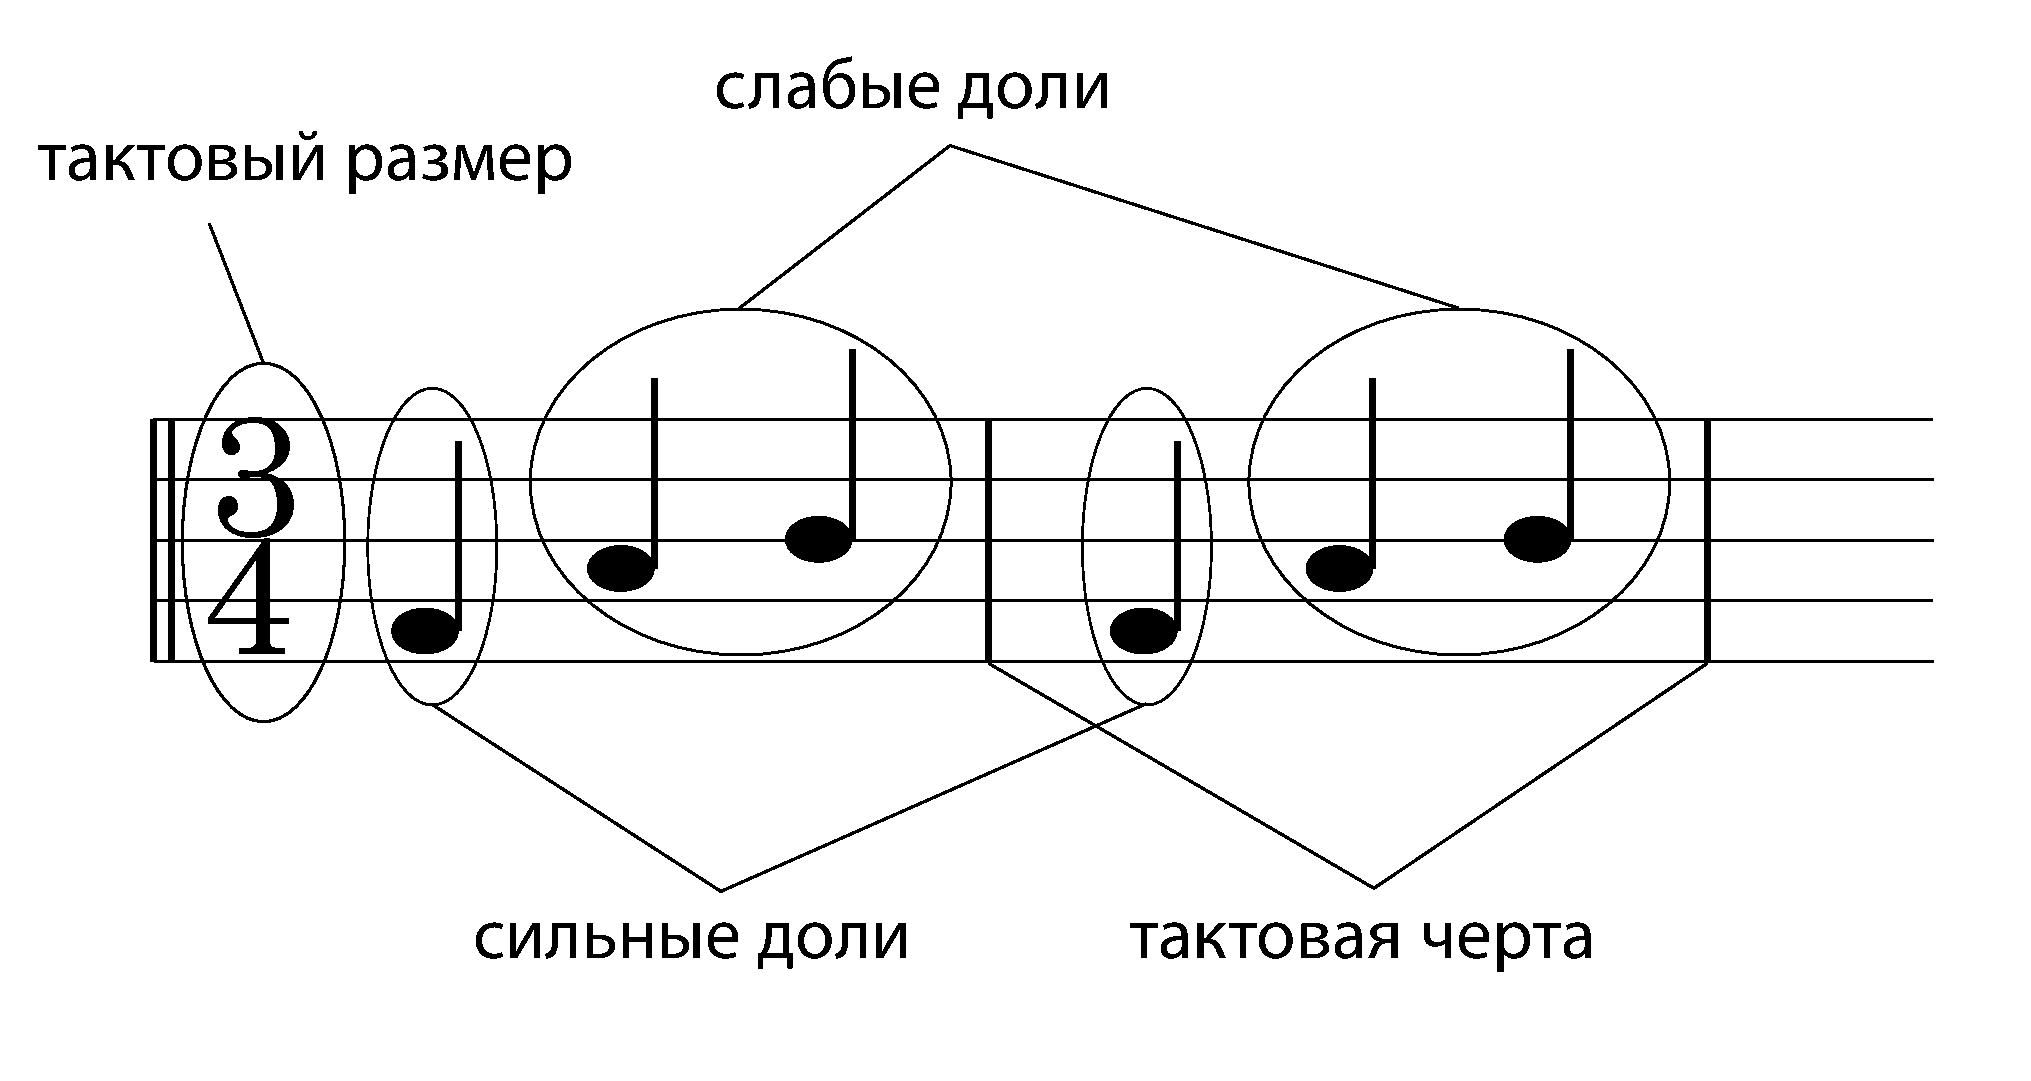
\includegraphics[scale=0.4]{svg/barlines.pdf}
	\caption{Обозначение метра}
	\label{img:meter}
\end{figure}

\newpage

Размер задает относительную длительность каждой доли. Например, размер <<3/4>> говорит о том, что в такте 3 доли, каждая из которых представлена четвертной нотой. Можно сказать, что размер -- числовое представление метра с указанием длительности каждой доли. Такт в свою очередь -- единица метра, начинающаяся с наиболее сильной доли и заканчивающаяся перед следующей равной ей по силе (рис.~\ref{img:meter}).

В данной работе не будут учитываться тонкости различия ритма и метра. Соответственно, для измерения ритма будет использоваться числовое представление метра в виде тактового размера.

\subsection{Проблема определения ритма и темпа}

Основной проблемой автоматического определения ритма и темпа музыки является наличие некоторых особенностей в музыкальных записях с живыми инструментами, затрудняющих это определение. Одна из таких особенностей -- это нечеткое попадание инструмента в ритмическую сетку. Такие небольшие отклонения на живых записях присутствуют всегда~\cite{quantize}. Они не заметны для уха человека, но могут осложнять автоматическое распознавание.

Также в некоторых случаях темп и ритм может изменяться в течение музыкального произведения. Пример переменного темпа приведен на рис.~\ref{img:aerials} (темп обозначается числами сверху в bpm). На рис.~\ref{img:master} приведен пример переменного ритма (размера).

\begin{figure}[h]
	\centering
	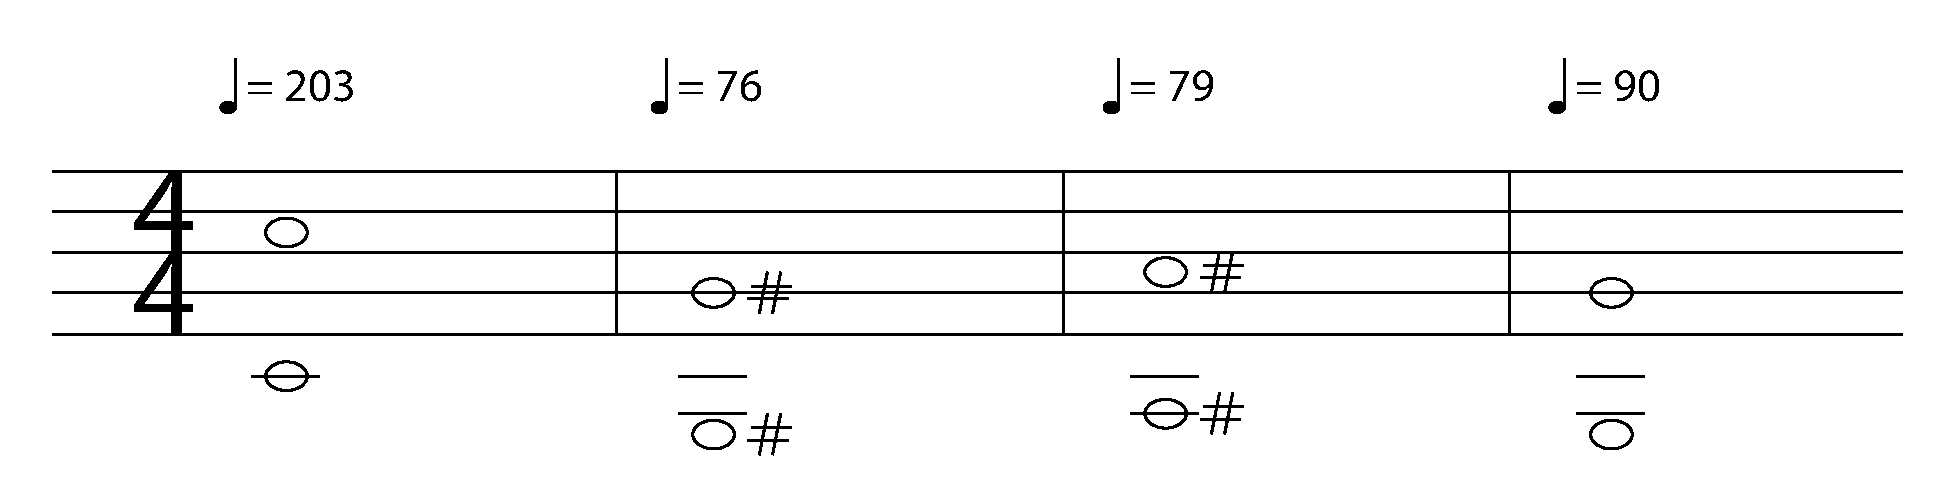
\includegraphics[scale=0.5]{svg/aerials.pdf}
	\caption{Пример переменного темпа (System of a down <<Aerials>>)}
	\label{img:aerials}
\end{figure}

\begin{figure}[h]
	\centering
	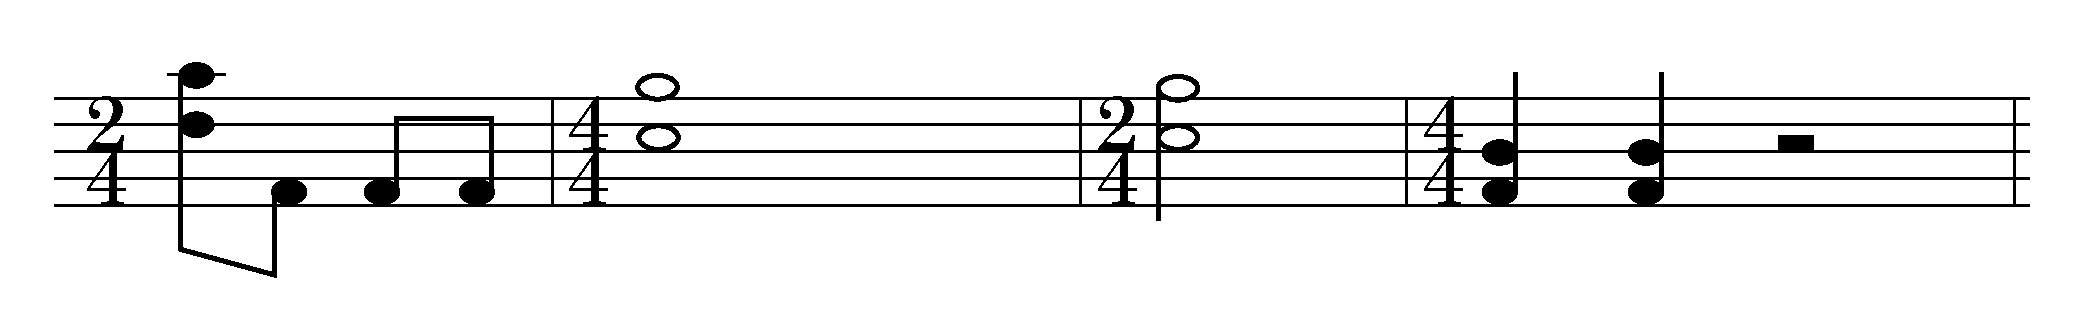
\includegraphics[scale=0.5]{svg/master.pdf}
	\caption{Пример переменного размера (Metallica <<Master of puppets>>)}
	\label{img:master}
\end{figure}

В качестве критериев сравнения рассматриваемых далее методов выделены следующие:

\begin{itemize}
	\item[---] точность результатов применения метода;
	\item[---] возможность определения переменного темпа и ритма;
	\item[---] ограничения на формат входного аудиофайла;
	\item[---] размер использовавшегося для обучения датасета (если обучение необходимо).
\end{itemize}

\subsection{Дискретное вейвлет-преобразование}

\subsubsection{Общие сведения}

Так как преобразование Фурье не позволяет получить частотно-временное представление сигнала, оно подходит только для стационарных сигналов (т. е. сигналов, частотное наполнение которых не меняется во времени). Большинство же реальных аудио-сигналов являются нестационарными. Основная же проблема оконного преобразования Фурье (ОПФ) заключается в невозможности получить произвольно точное частотно-временное представление сигнала, то есть нельзя определить для какого-то момента времени, какие спектральные компоненты присутствуют в сигнале. Эта проблема называется проблемой разрешения.

В качестве альтернативы ОПФ было разработано вейвлет-преобразование.

Основная идея вейвлет-преобразования -- это разделение сигнала на высокие и низкие частоты с помощью фильтров \cite{polikar}. После применения фильтров полученные низкие частоты снова пропускаются через два фильтра и т. д. При этом высокие частоты остаются неизменными. Эта операция называется декомпозицией.

На высоких частотах лучше разрешение по времени, а на низких -- по частоте.

Фильтры для высоких и низких частот определяются следующими уравнениями \cite{dwt}:

\begin{equation}\label{eq:highpass}
	y_{high}[k] = \sum_{n=-\infty}^{\infty} x[n] g[2k-n],
\end{equation}

\begin{equation}\label{eq:lowpass}
	y_{low}[k] = \sum_{n=-\infty}^{\infty} x[n] h[2k-n],
\end{equation}

где $x[n]$ -- пропускаемый через фильтр сигнал (последовательность), $h[n]$ и $g[n]$ -- импульсные характеристики (отклик на единичный импульс) низкочастотного и высокочастотного фильтров соответственно, $k$ и $n$ -- целые числа, соответствующие отсчетам (теорема отсчетов~\cite{samples}).

Выражение $2k-n$ в формулах \ref{eq:highpass} и \ref{eq:lowpass} позволяет обрезать сигнал, тем самым увеличив его масштаб в два раза (т.~к. половина частот удаляется в результате фильтрации)~\cite{polikar}.

Само ДВП (дискретное вейвлет-преобразование) описывается формулой:

\begin{equation}\label{eq:dwt}
	W(j, k) = \sum_{j}\sum_{k} x(k) 2^{-j/2} \psi(2^{-j}n-k),
\end{equation}

где $\psi(t)$ -- функция преобразования, называемая материнским вейвлетом, $j$ и $k$ связаны с параметрами сдвига $\tau$ (местоположение окна) и масштаба $s$ (величина, обратная частоте). $s = s_0^j$, $\tau = k s_0^j \tau_0$. В данном случае $s_0 = 2$, $\tau_0 = 1$.

\subsubsection{Определение ритма и темпа}

Алгоритм определения ритма с помощью ДВП основан на обнаружении наиболее заметных периодов сигнала.

Сигнал сначала раскладывается на несколько частотных полос с помощью ДВП. Для этого сигнал <<делится>> пополам на высокие и низкие частоты, после чего низкие частоты снова разделяются пополам и т.~д. Так продолжается до тех пор, пока не останутся два отсчета. Эта операция необходима, т.~к. для высоких частот можно точнее указать их временную позицию, а для низких -- их значение частоты~\cite{polikar}. После этого огибающая амплитуды во временной области каждой полосы извлекается отдельно. Это достигается за счет фильтрации нижних частот каждой полосы, применения полноволнового выпрямления и понижения частоты дискретизации \cite{dwt}. Затем огибающие каждой полосы суммируются и вычисляется автокорреляционная функция. Пики автокорреляционной функции соответствуют различным периодам огибающей сигнала.

Фильтрация нижних частот:

\begin{equation}
	y[n] = (1 - \alpha)x[n] - \alpha y[n],
\end{equation}

где $\alpha = 0,99$.

Полноволновое выпрямление:

\begin{equation}
	y[n] = abs(x[n]).
\end{equation}

Понижение частоты дискретизации:

\begin{equation}
	y[n] = x[kn].
\end{equation}

Нормализация в каждой полосе (удаление среднего значения) для исключения аномальных данных:

\begin{equation}
	y[n] = x[n] - E[x[n]],
\end{equation}

где $E[x[n]]$ -- среднее значение последовательности $x[n]$.

Автокорреляция:

\begin{equation}
	y[k] = \frac{1}{N} \sum_{n=0}^{N-1}x[n]x[n+k].
\end{equation}

Из результата берутся первые пять пиков автокорреляционной функции, после чего рассчитываются и добавляются в гистограмму соответствующие им периодичности в bpm. Этот процесс повторяется в процессе прохождения по сигналу. Периодичность, соответствующая наиболее заметному пику конечной гистограммы, является предполагаемым темпом аудиофайла в bpm.

Основными недостатками рассмотренного метода определения темпа являются неточные (в некоторых случаях даже ошибочные) результаты на музыке определенных жанров (например, на классической музыке), а также невозможность определить переменный темп.

\subsection{Скрытые модели Маркова}

\subsubsection{Стохастическое моделирование}

Как уже было упомянуто выше, практически во всех музыкальных записях имеет место небольшое отклонение нот от ритмической сетки. Рассматриваемый метод рассчитан именно на работу с такими случаями. Также в данном методе подразумевается, что входные данные представлены в формате MIDI (Musical Instrument Digital Interface, стандарт обмена данными между цифровыми музыкальными инструментами). В MIDI файлах указывается информация о высоте ноты, ее длительности и силе нажатия~\cite{midi}.

Исследования показывают, что отклонения нот можно смоделировать с помощью распределения Гаусса относительно их идеальной длительности~\cite{hmm}. Тогда, если $i$ -- идеальная длительность ноты (<<намерение>>) в момент времени $t$, то ее исполненная длительность $x_t$ моделируется функцией плотности вероятности $f_i(x_t)$.

Пусть $Q = \{q_1, q_2, ..., q_N\}$ -- последовательность <<намерений>> в соответствующие моменты времени. Тогда наблюдаемая последовательность длительностей $X = \{x_1, x_2, ..., x_N\}$ определяется как:

\begin{equation}
	P(X|Q) = \prod_{t=1}^N f_{q_t}(x_t).
\end{equation}

В данном методе используются два типа моделей генерации ритмических рисунков для получения возможных ритмов:

\begin{itemize}
	\item[---] n-граммная модель (длина ноты предсказывается исходя из предыдущих n-1 нот в вероятностном смысле. Эта модель охватывает любые ритмические рисунки и может выдавать точную вероятность);
	\item[---] <<ритмический словарь>> (состоит из всех известных ритмических рисунков за единицу времени. Хорошо представляет известные ритмические рисунки, в то время как неизвестные заменяются аналогичными существующими ритмами).
\end{itemize}

Обе модели можно представить в виде вероятностных сетей перехода состояний, где каждое состояние связано с предполагаемой длительностью ноты. Вероятность того, что номер состояния изменится в последовательности $Q = \{q_1, q_2, ..., q_N\}$ определяется как $P(Q) = p_{q_0} \prod_{t=1}^N a_{q_{t-1}q_t}$, где $p_i$ -- вероятность изначального нахождения в состоянии $i$, а $a_{ij}$ -- вероятность перехода из состояния $i$ в состояние $j$.

Колеблющиеся длительности и возможные последовательности нот могут быть объединены в рамках скрытой модели Маркова как вероятности перехода $A = \{a_{ij}\}$ и наблюдаемые вероятности $B = \{b_i(x_t)\}$ соответственно. В таком случае вероятность наблюдения последовательности длительностей $X$ определяется как:

\begin{equation}
	P(X) = P(X|Q)P(Q).
\end{equation}

\subsubsection{Определение ритма}

Задача заключается в том, чтобы найти временную последовательность $Q$ номеров состояний, которая дает максимальную апостериорную вероятность $P(Q|X)$ при заданной последовательности наблюдаемых длительностей $X$~\cite{hmm}.

По теореме Байеса:

\begin{equation}\label{eq:bayes}
	P(Q|X) = \frac{P(X|Q)P(Q)}{P(X)}.
\end{equation}

Значит, максимизация апостериорной вероятности эквивалентна нахождению $argmax P(X|Q)P(Q)$ среди всех возможных $Q$.

Оптимальная последовательность состояний находится с помощью алгоритма Витерби для поиска наилучшего пути в вероятностной сети переходов.

Основной недостаток представленного метода заключается в необходимости входных данных быть в формате MIDI. Также к недостаткам можно отнести периодические неточности в результатах. Например, музыкальные фрагменты с разным темпом (к примеру, 116 bpm и 127 bpm) могут быть определены как имеющие одинаковый темп (в данном случае 120 bpm~\cite{hmm}).

\subsection{Байесовское иерархическое моделирование}

\subsubsection{Общие сведения}

Байесовская иерархическая модель - это метод статистического анализа, который использует байесовский подход для оценки параметров. Она состоит из нескольких уровней, где каждый уровень описывает определенный аспект данных~\cite{kubler_pymc3}.

Для каждого уровня иерархии определяются соответствующие параметры, которые описывают данные. Для оценки параметров используются априорные распределения, которые описывают предположения об этих параметрах до получения данных. Затем с помощью формулы~\ref{eq:bayes} оцениваются параметры модели, учитывая как данные ($P(X|Q)$), так и априорные распределения ($P(Q)$). Таким образом, байесовская иерархическая модель позволяет учитывать неопределенность в данных и параметрах модели, а также учитывать различные уровни влияния на данные.

Термин $P(X|Q)$ играет две роли в статистике, в зависимости от контекста~\cite{bayes_hier}. Когда она рассматривается как функция от $X$ для известного $Q$, то она называется \textbf{функцией массы вероятности}. Функция массы вероятности описывает вероятность любого исхода $X$ при заданном значении $Q$. Но этот термин также можно рассматривать как функцию параметра $Q$ для фиксированного $X$. В этом случае она называется \textbf{функцией правдоподобия} и описывает вероятность определенного значения параметра $Q$ при заданном фиксированном значении $X$. В теореме Байеса используется апостериорное распределение ($P(Q|X)$) как функция параметра $Q$. Следовательно, $P(X|Q)$ рассматривается как правдоподобие параметра $Q$, а не масса вероятности $X$.

Член $P(X)$ является константой по отношению к $Q$ и служит нормирующим числом, которое гарантирует, что апостериорная вероятность не превышает 1.

Чтобы выполнить байесовский анализ, необходимо выбрать априорное распределение $P(Q)$. Этот выбор отражает мнение о возможных значениях $Q$ до сбора данных.

Когда априорная и апостериорная вероятность относятся к одному и тому же распределению, они называются \textbf{сопряженными}~\cite{bayes_hier}. Сопряженные значения удобны, они часто облегчают получение апостериорных распределений. Однако сопряженность вовсе не обязательна для байесовского анализа.

\subsubsection{Определение темпа и ритма}

В случае с темпом музыки формула~\ref{eq:bayes} принимает вид:

\begin{equation}\label{eq:bayes_tempo}
	P(t|d) = \frac{P(d|t)P(t)}{P(d)},
\end{equation}

где $d$ -- это собранные данные с известным темпом (датасет), а $t$ -- искомый темп.

Аналогично и с ритмом (тактовым размером).

Однако темп музыки имеет также некоторую корреляцию с жанром. Поэтому в таком случае лучше всего применять иерархический вариант рассмотренной выше байесовской модели. Тогда на первом уровне будут располагаться так называемые \textbf{гипераприорные} распределения~\cite{kubler_pymc3} для темпа и для жанра ($P(t)$ и $P(g)$ соответственно). На основе этих распределений вычисляются параметры, располагающиеся на втором уровне и необходимые для задания распределения функции правдоподобия (likelihood\_params) (см. рис.~\ref{img:hbm}). На третьем же уровне находится функция правдоподобия, которая задается на основе вычисленных ранее параметров.

\begin{figure}[h]
	\centering
	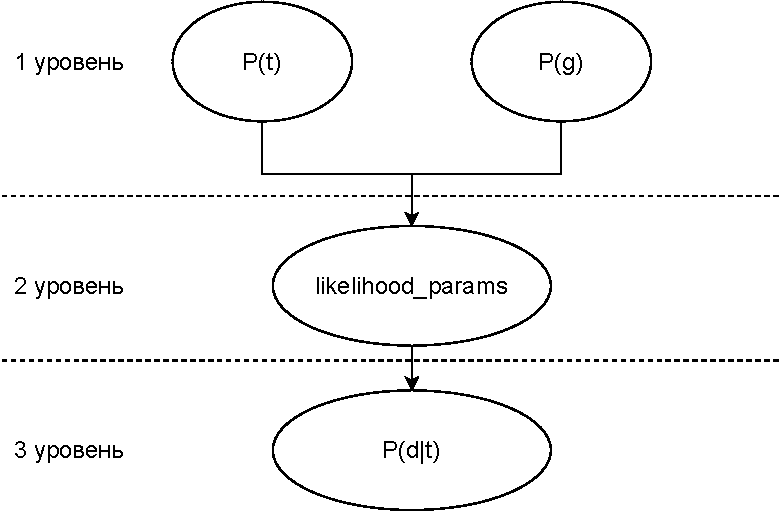
\includegraphics[scale=0.9]{svg/hierarchical.pdf}
	\caption{Схема иерархической байесовской модели}
	\label{img:hbm}
\end{figure}

Таким образом, байесовское иерархическое моделирование позволяет немного увеличить точность определения ритма по сравнению с марковскими моделями (примерно на 2\%~\cite{bayesian}). Однако главным недостатком байесовского моделирования является возможное неправильное задание априорного распределения. Также к недостаткам можно отнести определение только постоянного темпа и ритма.

\subsection{Использование сверточных нейросетей}

\subsubsection{Представление сигнала}

Сигнал представляется в виде спектрограммы по шкале мела, чтобы снизить объем данных, который должен быть обработан нейросетью (мел, от слова <<мелодия>>, - психофизическая (субъективная) единица высоты звука~\cite{mels}). Шкала мела выбрана вместо линейной шкалы из-за ее связи с человеческим восприятием и диапазонами частот инструментов.

Чтобы создать спектрограмму, сигнал конвертируется в моно, его дискретизация понижается до 11025~Гц, после чего используются полуперекрывающиеся окна из 1024 отсчетов~\cite{cnn}. Это эквивалентно частоте кадров 21,5~Гц, что (согласно теореме отсчетов) достаточно для представления темпа до 646 bpm. Каждое окно преобразуется в 40-полосный спектр в шкале мел, охватывающий диапазон от 20 до 5000~Гц. В качестве длины спектрограммы выбрано 256 кадров, что примерно равняется 11,9~с.

\subsubsection{Архитектура сети}

Архитектура рассматриваемой сети представлена на рис.~\ref{img:cnn}.

Сначала входные данные обрабатываются тремя сверточными слоями, каждый из которых состоит из 16 фильтров размера 1х5. С помощью этих фильтров сопоставляется ритмическая структура сигнала.

После этого идут четыре модуля с несколькими фильтрами. Каждый из модулей состоит из среднего слоя пулинга (<<avg pooling>>), шести параллельных сверточных слоев с фильтрами разных размеров (от 1х32 до 1х256), слоя конкатенации и т.~н. <<узкого>> (<<bottle-neck>>) слоя, предназначенного для уменьшения размерности. С помощью этих модулей достигаются две цели:

\begin{enumerate} 
	\item Пулинг по оси частот для суммирования диапазонов мел.
	\item Сопоставление сигнала с различными фильтрами, способными обнаруживать длительные временные зависимости.
\end{enumerate}

Чтобы классифицировать свойства, полученные из сверточных слоев, добавляются два полносвязных слоя (по 64 единицы каждый), за которыми следует выходной слой с 256 единицами. Выходной слой использует softmax в качестве функции активации, а все остальные слои используют ELU~\cite{elu}. Каждому сверточному или полносвязному слою предшествует пакетная нормализация~\cite{batch}. Первому полносвязному слою также предшествует слой отсева с $p = 0,5$ (<<dropout>>) для противодействия переобучению.

\begin{figure}[h]
	\centering
	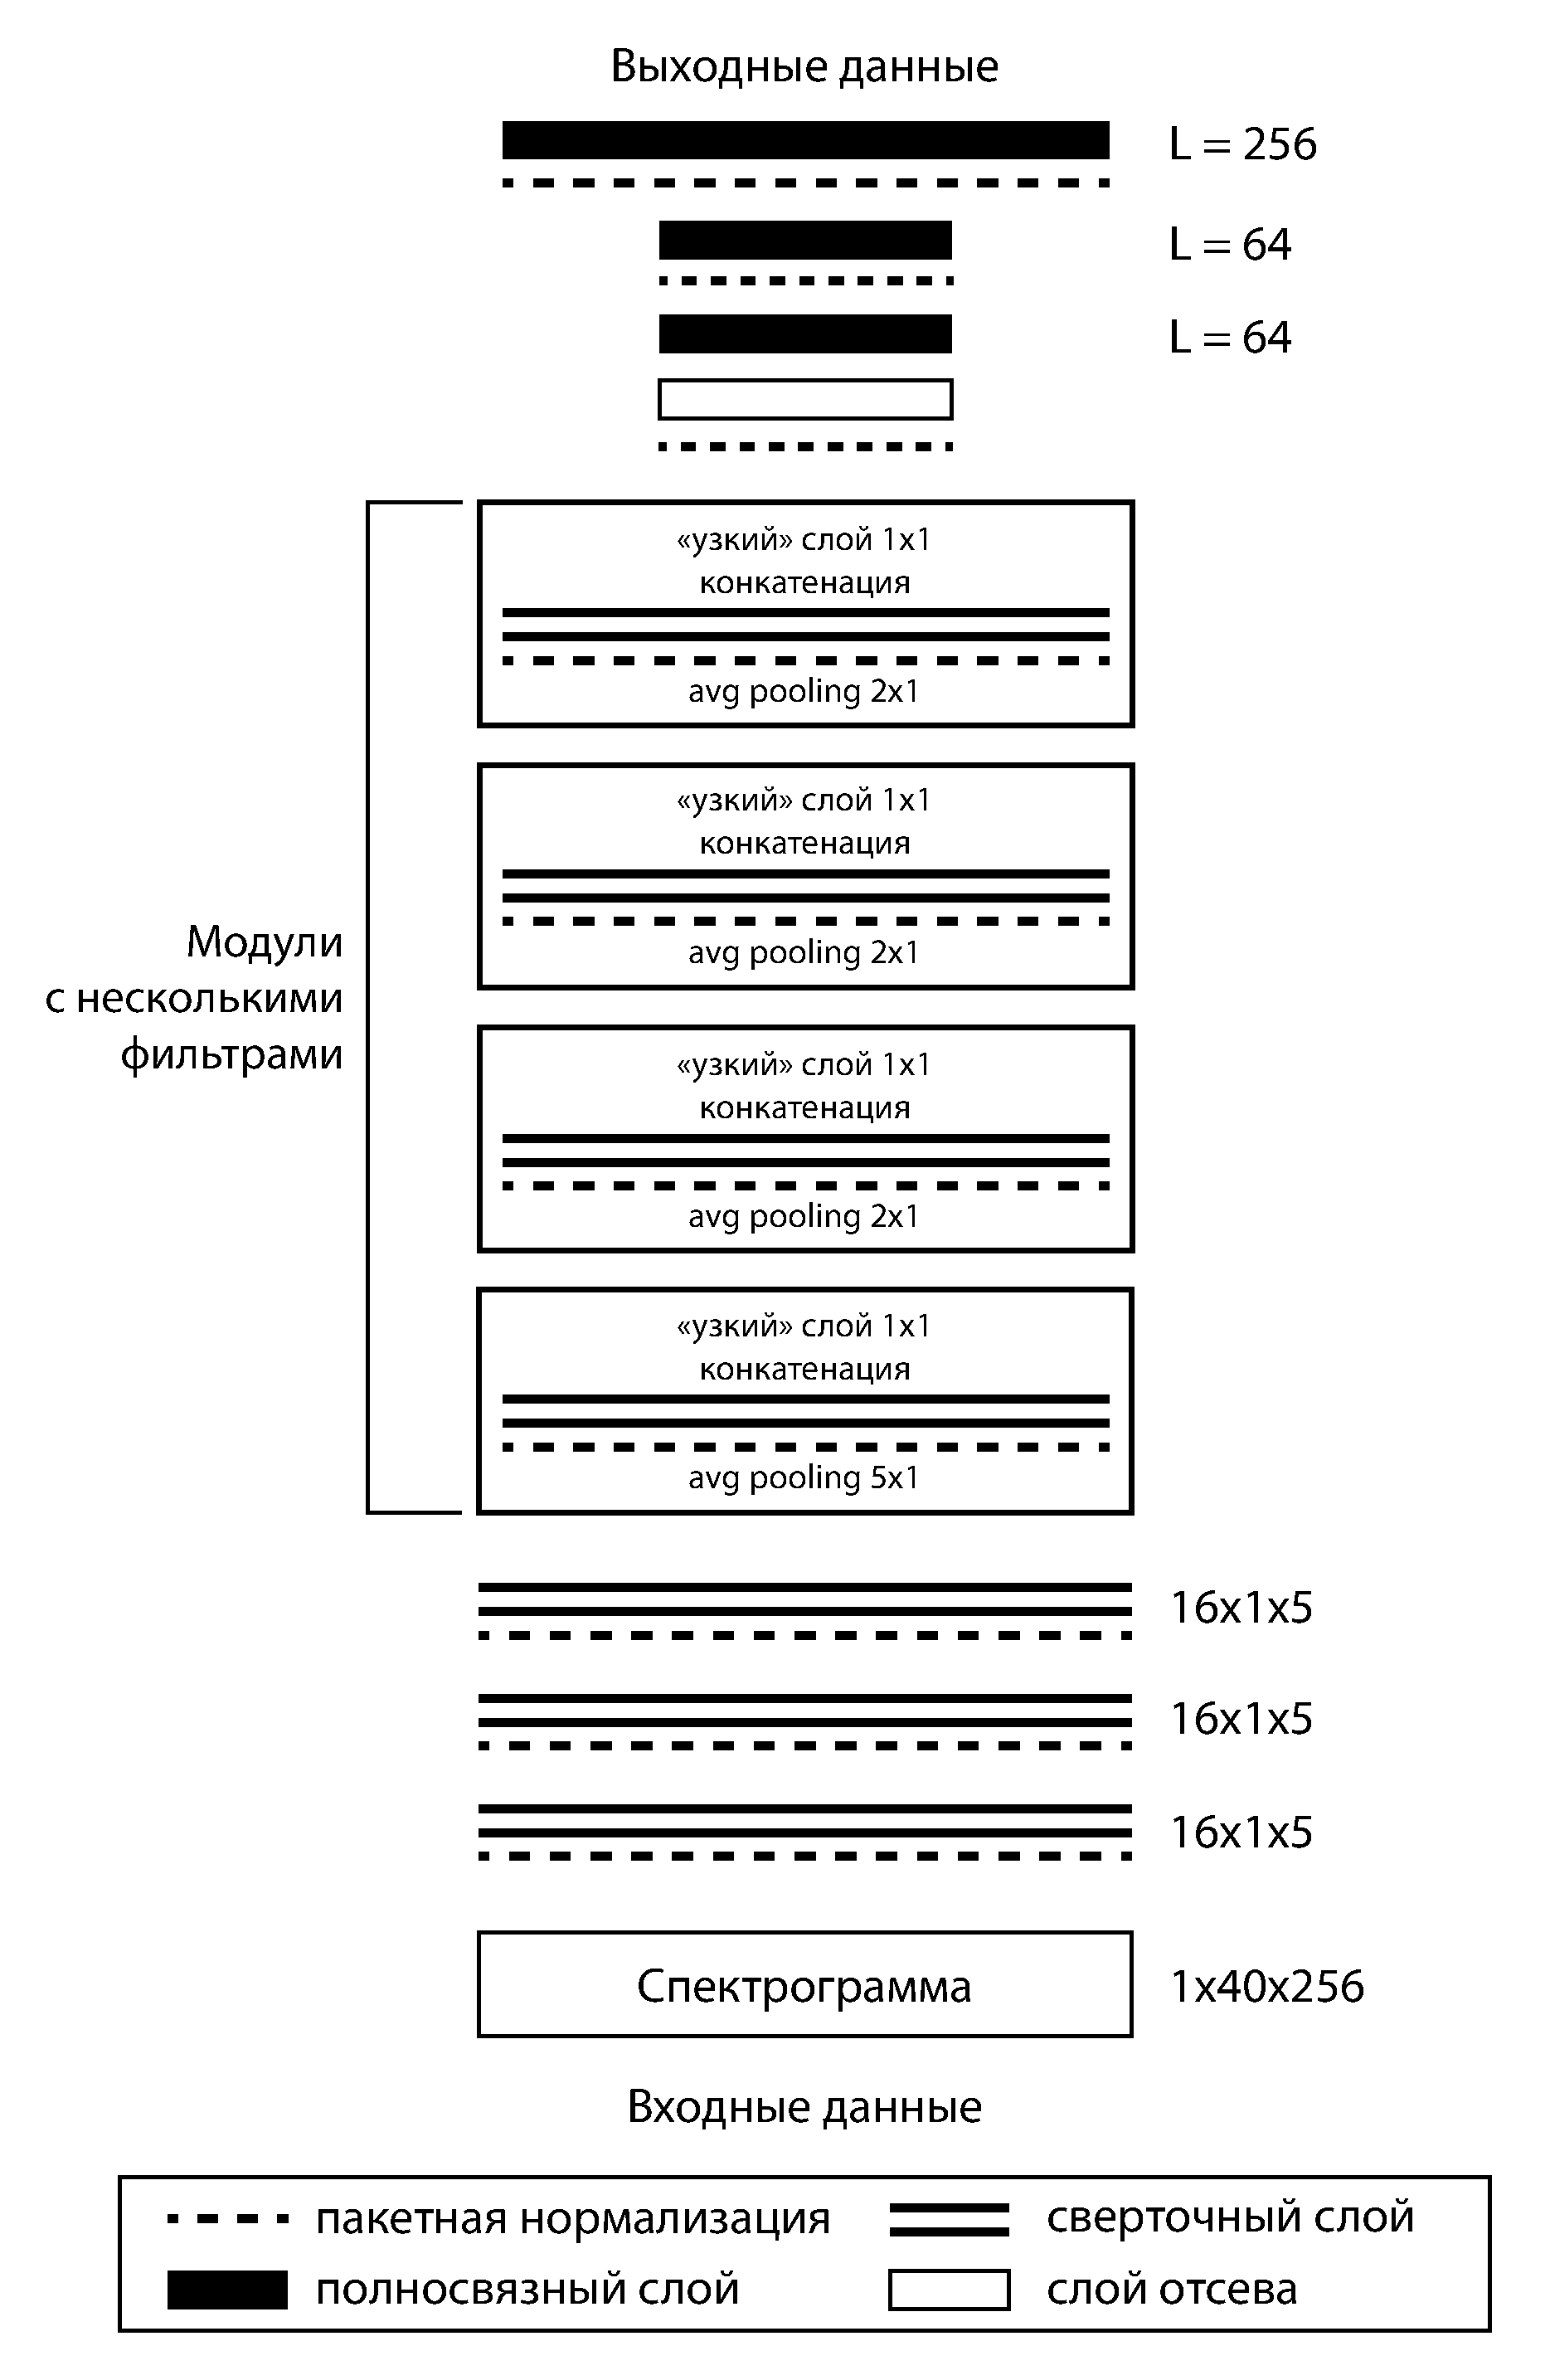
\includegraphics[scale=0.38]{svg/cnn.pdf}
	\caption{Схема архитектуры нейросети}
	\label{img:cnn}
\end{figure}

Всего сеть имеет 2921042 обучаемых параметра.

В результате выбирается один из 256 вариантов темпа от 30 до 285 bpm.

Таким образом, сверточные нейросети позволяют определять темп с достаточно высокой точностью (процент правильных оценок с допустимой погрешностью в 4\%) (до 92\% на основе комбинированной выборки, состоящей из аудиофайлов различных жанров с темпом от 44 до 216 bpm~\cite{cnn}). Также данный метод можно использовать и при определении глобального темпа, не только для фрагментов.

Но он по-прежнему не позволяет определить переменный темп, а также не предназначен для определения ритма. Помимо этого нейросетевые методы имеют такие недостатки, как необходимость обучающих датасетов больших объемов, зависимость от исходных данных и долгое время обучения.

\subsection{Сравнение методов}

По результатам рассмотрения перечисленных выше методов была составлена таблица \ref{tbl:compare}.

Как видно из таблицы, ни один метод в своем изначальном варианте не предполагает определение переменного темпа и ритма. Однако метод скрытых марковских моделей при небольшой модификации может позволить определить переменный темп и ритм~\cite{hmm}.

Также стоит заметить, что все методы, кроме ДВП, содержат обучаемые параметры. В скрытых марковских моделях -- это множество $\{a_{ij}\}$, а в байесовском иерархическом моделировании -- множество $\{\pi_{kk'}\}$. В обоих методах обучение происходит с помощью статистической оценки. Размеры датасетов в таблице были указаны исходя из данных, использовавшихся для обучения соответствующих моделей в исследованиях.

\begin{table}[h!]
	\begin{center}
		\caption{\label{tbl:compare}Сравнение рассмотренных методов}
		\begin{tabular}{|p{2.5cm}|p{3cm}|p{3cm}|p{3cm}|p{3cm}|}
			\hline
			Метод & Точность результатов & Переменный темп и ритм & Формат входного аудиофайла & Размер использовавшегося датасета (кол-во аудиофайлов) \\\hline
			ДВП & Примерно $65\%$ (13 верных из 20)~\cite{dwt} & Не определяются  & Нет ограничений & Обучение не требуется\\\hline
			Скрытые марковские модели & Примерно $80\%$ (при допустимой погрешности $4\%$) & Могут определяться при модификации метода & MIDI & 88~\cite{hmm}\\\hline
			На основе БИМ* & Примерно $82\%$ & Не определяются  & Нет ограничений & 100~\cite{bayesian}\\\hline
			Сверточная нейросеть & До $92\%$  & Не определяются  & Нет ограничений & 8596~\cite{cnn}\\\hline
		\end{tabular}
	\end{center}
\end{table}

\newpage

*БИМ -- байесовское иерархическое моделирование.

\subsection*{Выводы}

В этом разделе была проанализирована предметная область и сформулирована проблема. А также была проведена классификация и сравнение основных существующих методов решения поставленной задачи, которое показало, что метод на основе байесовского иерархического моделирования дает достаточно высокую точность результатов, при этом не имея ограничений на формат входного аудиофайла и не требуя много времени на обучение.

Таким образом, необходимо разработать метод на основе байесовского иерархического моделирования, способный определять переменные темп и ритм музыки. Для этого требуется составить модели, которые будут использовать статистические данные о музыке, такие как темп и тактовый размер. Модель для определения темпа должна также учитывать жанр анализируемой музыки. Составленные модели должны быть обучены на наборе данных, включающих в том числе различные жанры~\cite{dataset}. После обучения моделей, они должны быть протестированы на новых данных, чтобы оценить их точность и эффективность.

На рисунке~\ref{img:idef_0} представлена формализация постановки задачи в виде\\ IDEF0-диаграммы.

\begin{figure}[h]
	\centering
	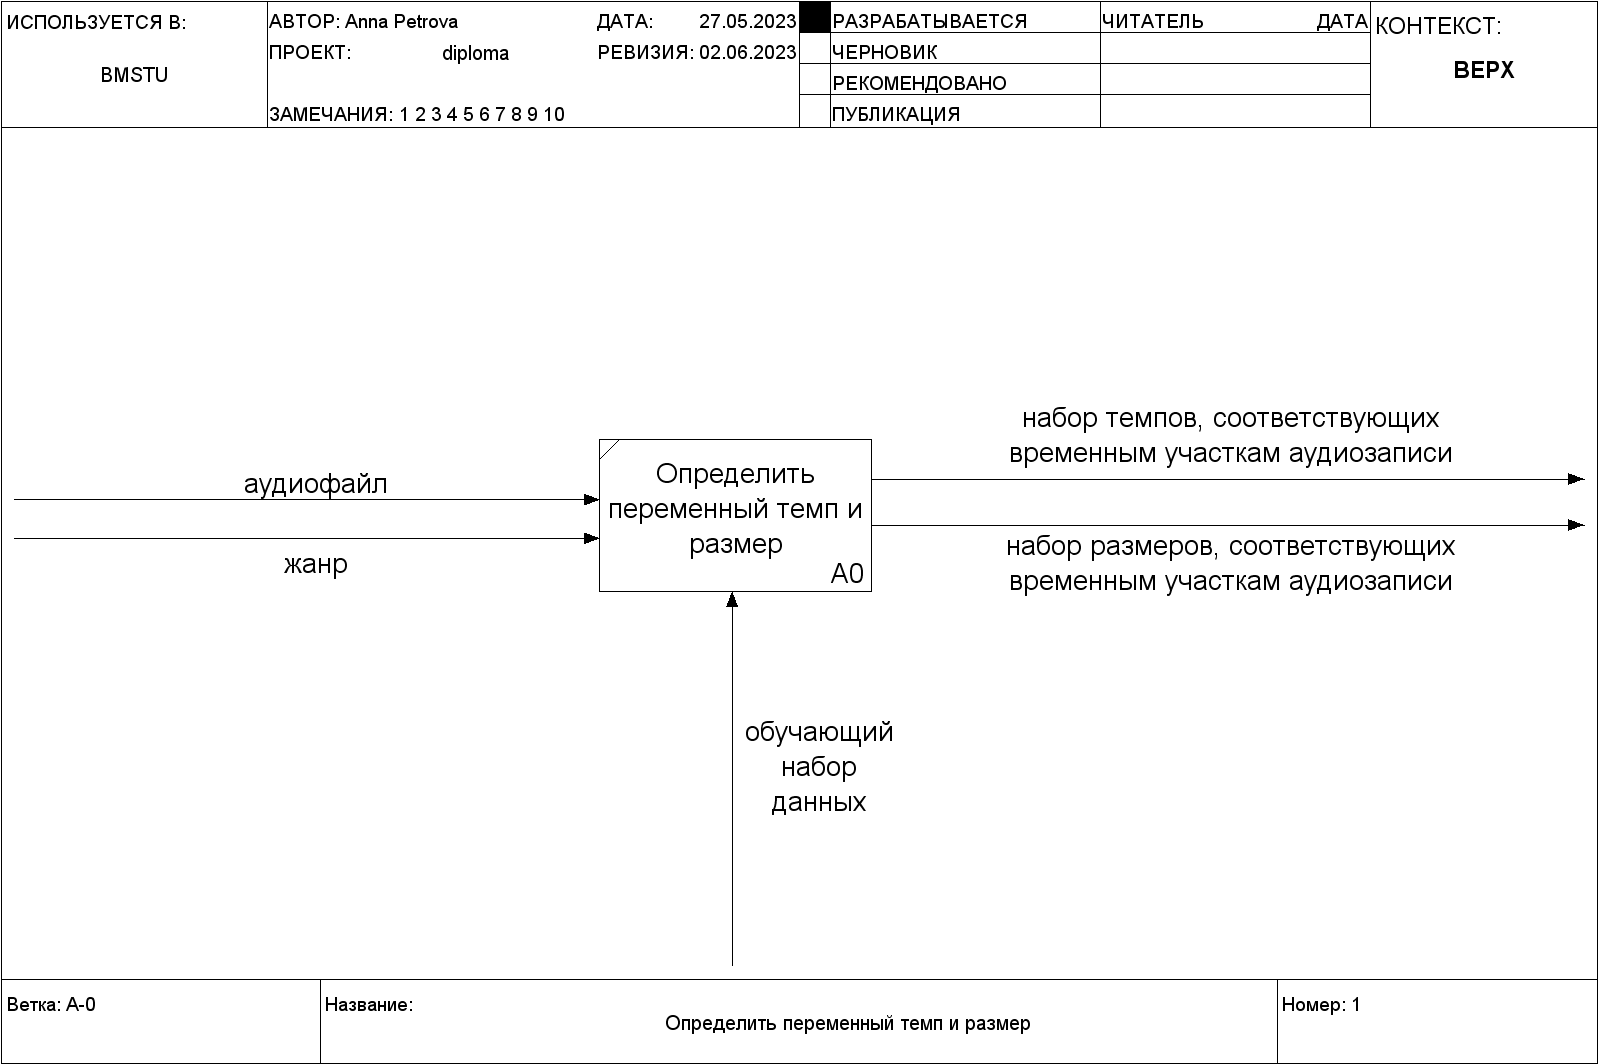
\includegraphics[scale=0.3]{inc/img/idef_analit.png}
	\caption{IDEF0 нулевого уровня для поставленной задачи}
	\label{img:idef_0}
\end{figure}

Входные данные:

\begin{itemize}
	\item[---] аудиофайл;
	\item[---] жанр музыки (строка).
\end{itemize}

Выходные данные:

\begin{itemize}
	\item[---] набор темпов, соответствующих временным участкам аудиозаписи (целые числа, в BPM);
	\item[---] набор тактовых размеров, соответствующих временным участкам аудиозаписи (обыкновенные дроби в формате <<a/b>>).
\end{itemize}

Ограничения:

\begin{itemize}
	\item[---] загружаемые аудиофайлы должны быть в формате mp3;
	\item[---] знаменатель тактового размера принимается равным 4.
\end{itemize}

%\section{Конструкторский раздел}
\setcounter{figure}{0}
\setcounter{table}{0}

\subsection{Определение переменного темпа}

На рисунках \ref{img:tempo_0} -- \ref{img:tempo_3} приведены IDEF0-диаграммы для метода определения переменного темпа музыки.

\begin{figure}[h]
	\centering
	\includegraphics[scale=0.25]{inc/img/tempo_idef/01_A-0.png}
	\caption{IDEF0 нулевого уровня}
	\label{img:tempo_0}
\end{figure}

Для адаптации используемого метода к определению переменного темпа музыки анализируемый аудиофайл разделяется на равные фрагменты. Опытным путем было выявлено, что оптимальной длиной фрагментов является 5 секунд. Если взять более короткие фрагменты, то методу начинает не хватать данных для определения темпа из-за слишком маленькой длины аудио. При этом если разделять на более крупные фрагменты, то увеличивается риск пропуска изменений темпа.

\begin{figure}[h]
	\centering
	\includegraphics[scale=0.25]{inc/img/tempo_idef/02_A0.png}
	\caption{Определение переменного темпа}
	\label{img:tempo_1}
\end{figure}

При реализации байесовской иерархической модели в качестве априорного распределения темпа анализируемой музыки было выбрано равномерное распределение с границами от минимального возможного темпа до максимального. Границы темпа выбираются на основе указанного жанра музыки. Такое распределение было выбрано, так как на данном этапе, за неимением каких-либо других характеристик указанного аудиофайла, предполагается, что все темпы для него в заданных пределах равновероятны.

Коэффициенты жанров необходимы для корректировки получаемой оценки темпа в зависимости от жанра музыки. Если коэффициент отрицательный, то темп должен быть уменьшен, если положительный -- увеличен. В качестве априорного распределения коэффициентов для всех жанров было выбрано нормальное распределение с математическим ожиданием, равным 0, и дисперсией, равной 1. Такой выбор связан с тем, что чаще всего разница между темпами в зависимости от жанра не слишком большая. Это означает, что корректирующие коэффициенты с большей вероятностью находятся в <<районе>> нуля. При этом 0 является <<нейтральным>> коэффициентом, т.~е. не влияет на полученную оценку темпа.

На основе информации из датасета было выявлено, что распределение темпов различной музыки близко к нормальному (рис.~\ref{img:bpm_distribution}).

\begin{figure}[h]
	\centering
	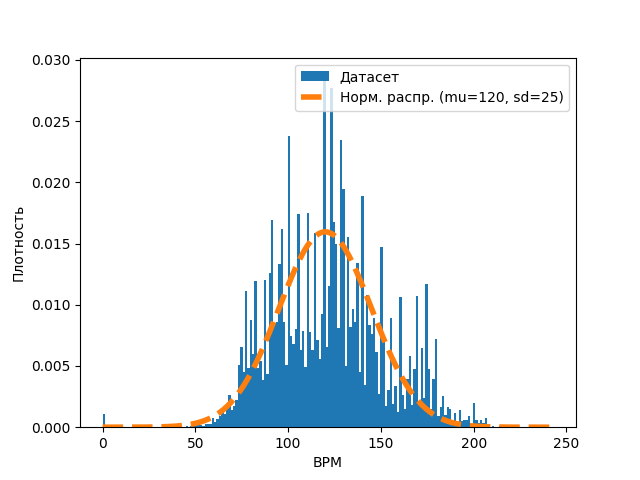
\includegraphics[scale=0.7]{../graphs/bpm_distribution.png}
	\caption{Распределение темпов музыки из датасета}
	\label{img:bpm_distribution}
\end{figure}

Поэтому в качестве распределения функции правдоподобия темпа было выбрано нормальное распределение. Математическое ожидание для каждого жанра для этого распределения рассчитывается на основе мат. ожидания и дисперсии априорного распределения темпа и априорных распределений коэффициентов жанров по формуле:

\begin{equation}
	\mu = \mu_{\text{prior}} + \text{coef} * \sigma_{\text{prior}},
\end{equation}

где $\mu_{\text{prior}}$ -- мат. ожидание априорного распределения темпа, $\sigma_{\text{prior}}$ -- дисперсия априорного распределения темпа, coef -- априорный коэффициент текущего жанра.

В качестве дисперсии при этом используется дисперсия априорного распределения темпа.

\begin{figure}[h]
	\centering
	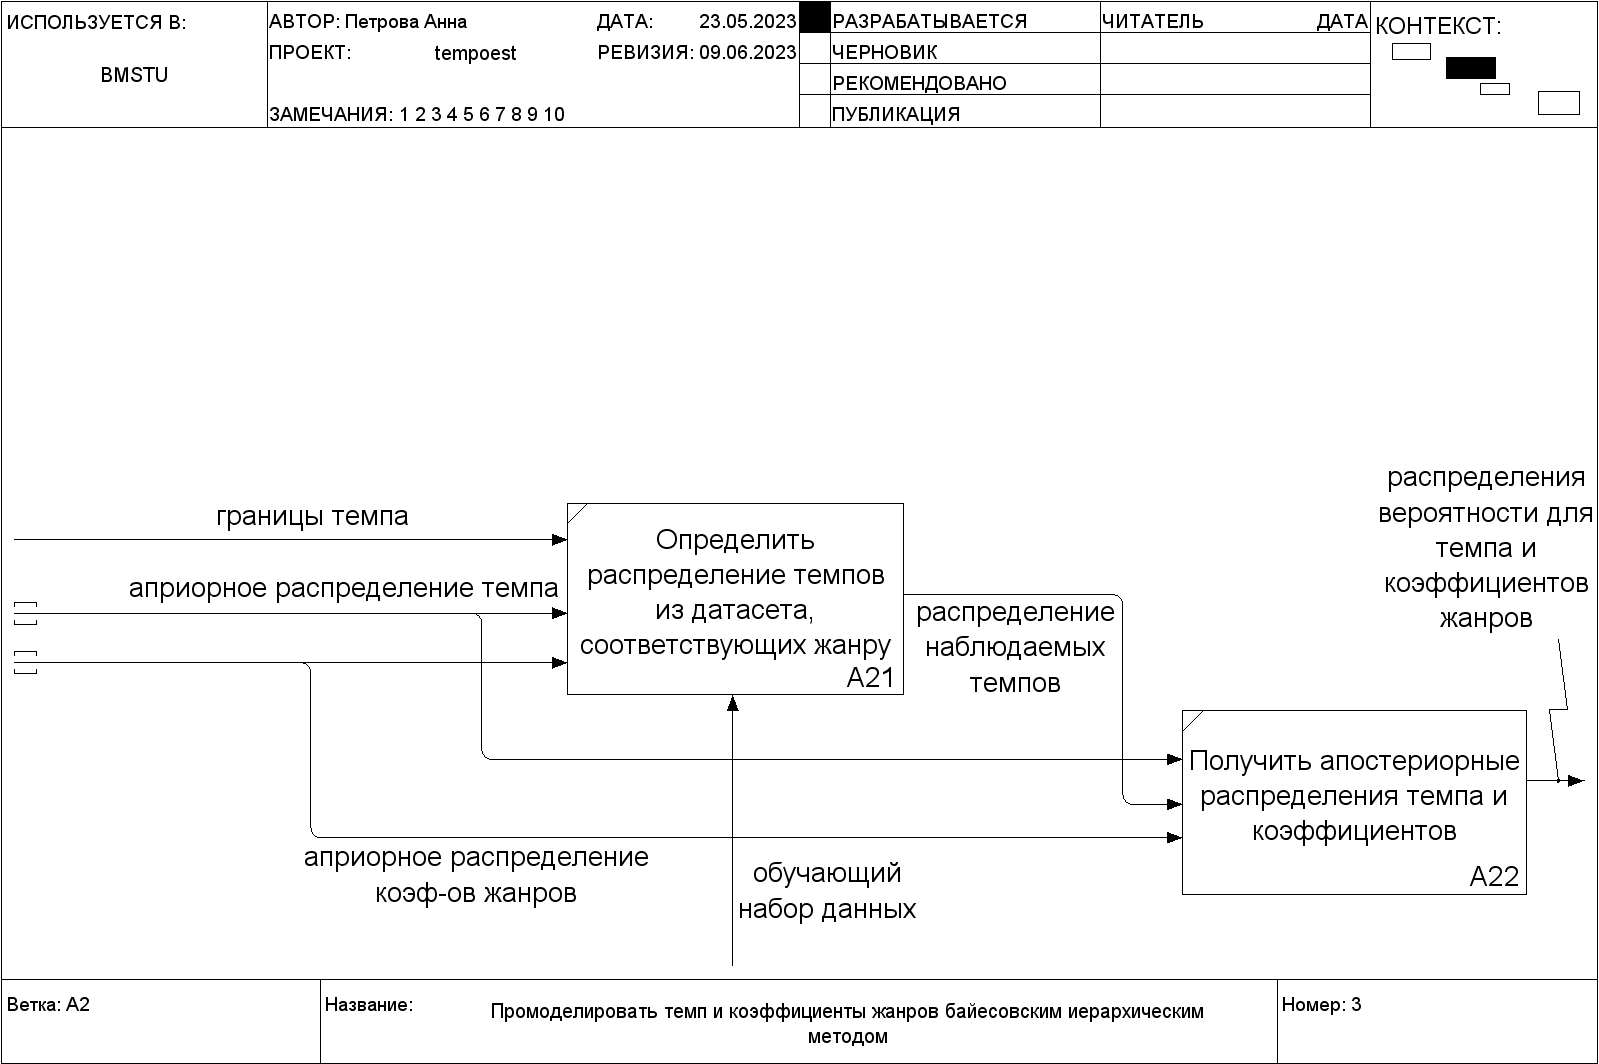
\includegraphics[scale=0.25]{inc/img/tempo_idef/03_A2.png}
	\caption{Байесовское моделирование}
	\label{img:tempo_2}
\end{figure}

Важно заметить, что в самой байесовской модели не используется анализируемый аудиофайл. В результате подсчета модели получаются апостериорные распределения темпа для заданного жанра в заданных границах и коэффициентов жанров.

После моделирования для каждого фрагмента аудиофайла рассчитывается примерный диапазон возможных темпов. Для этого сначала определяются так называемые <<силы нажатия>> на ноты, то есть амплитуды сигнала во временной области, после чего определяется приблизительное значение темпа на основе корреляции этих амплитуд. Далее относительно найденного темпа делается разброс значений в определенном интервале. Этот диапазон <<накладывается>> на полученное байесовским моделированием распределение темпа, и получается наиболее вероятный темп (максимум плотности распределения) в данном диапазоне (tempo) (рис.~\ref{img:res_tempo}).

После этого среди апостериорных распределений коэффициентов жанров находится распределение для указанного жанра. В этом распределении ищется наиболее вероятный коэффициент (coef). После чего применяется формула:

\begin{equation}
	\text{result} = \text{tempo} + \text{coef} * \sigma_{\text{prior}}.
\end{equation}

\begin{figure}[h]
	\centering
	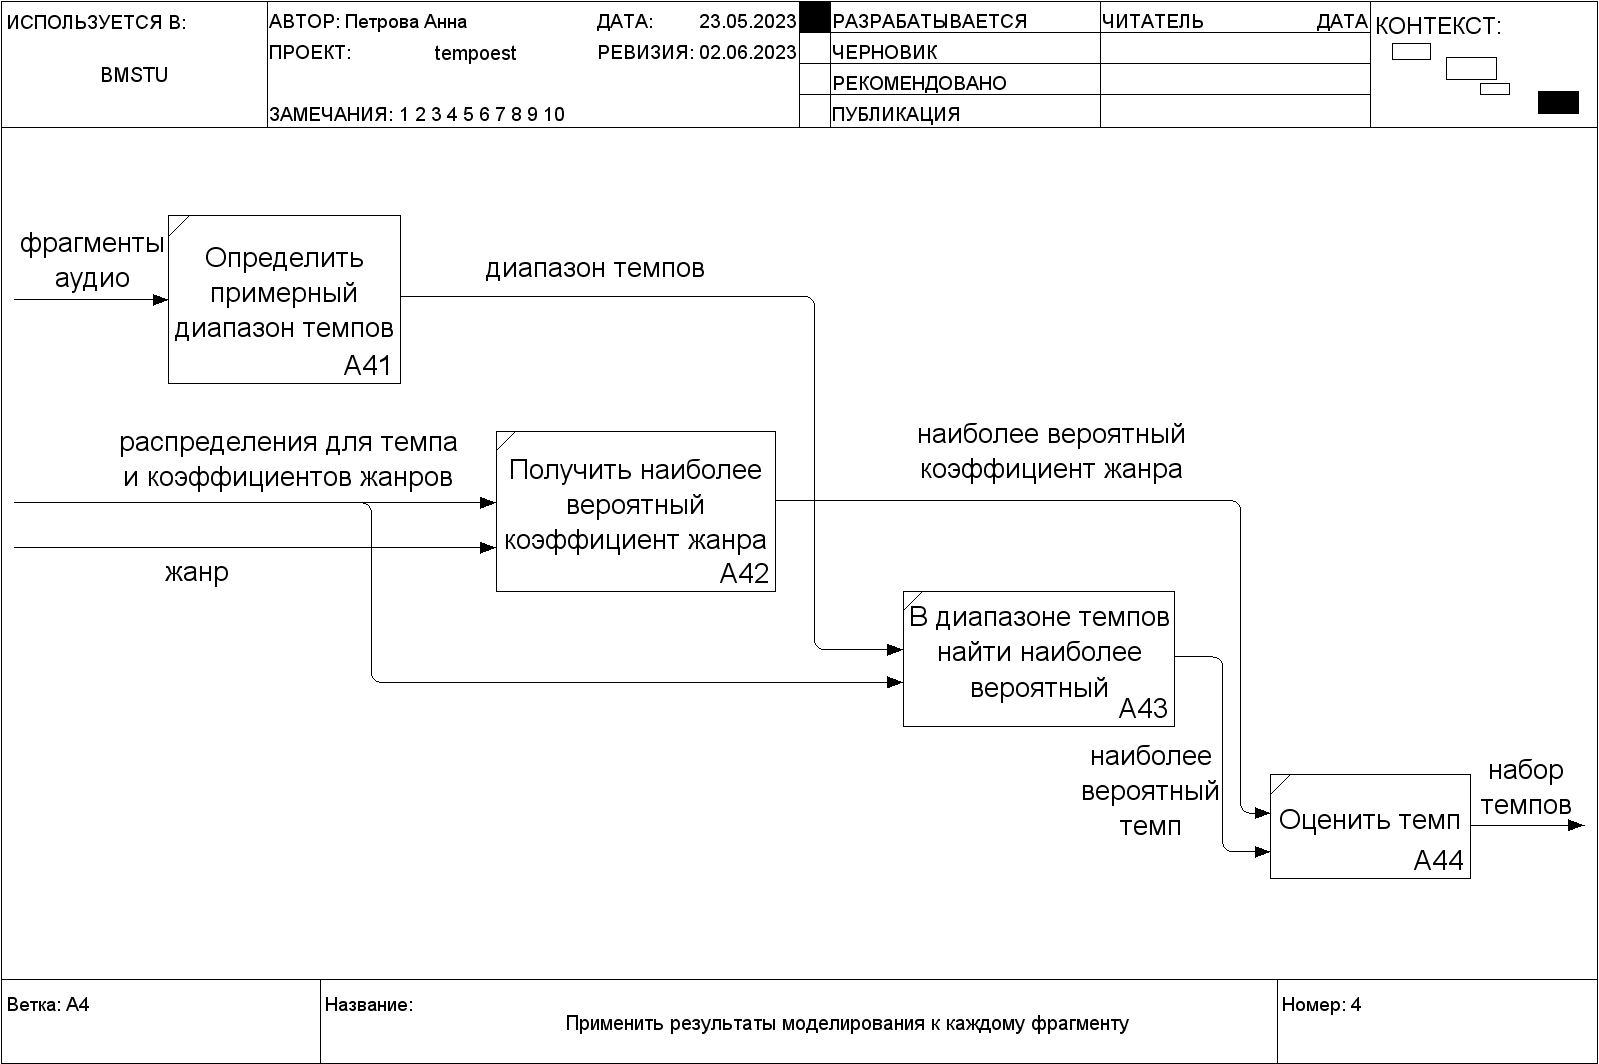
\includegraphics[scale=0.25]{inc/img/tempo_idef/04_A4.png}
	\caption{Применение результатов к фрагментам аудио}
	\label{img:tempo_3}
\end{figure}

\begin{figure}[h]
	\centering
	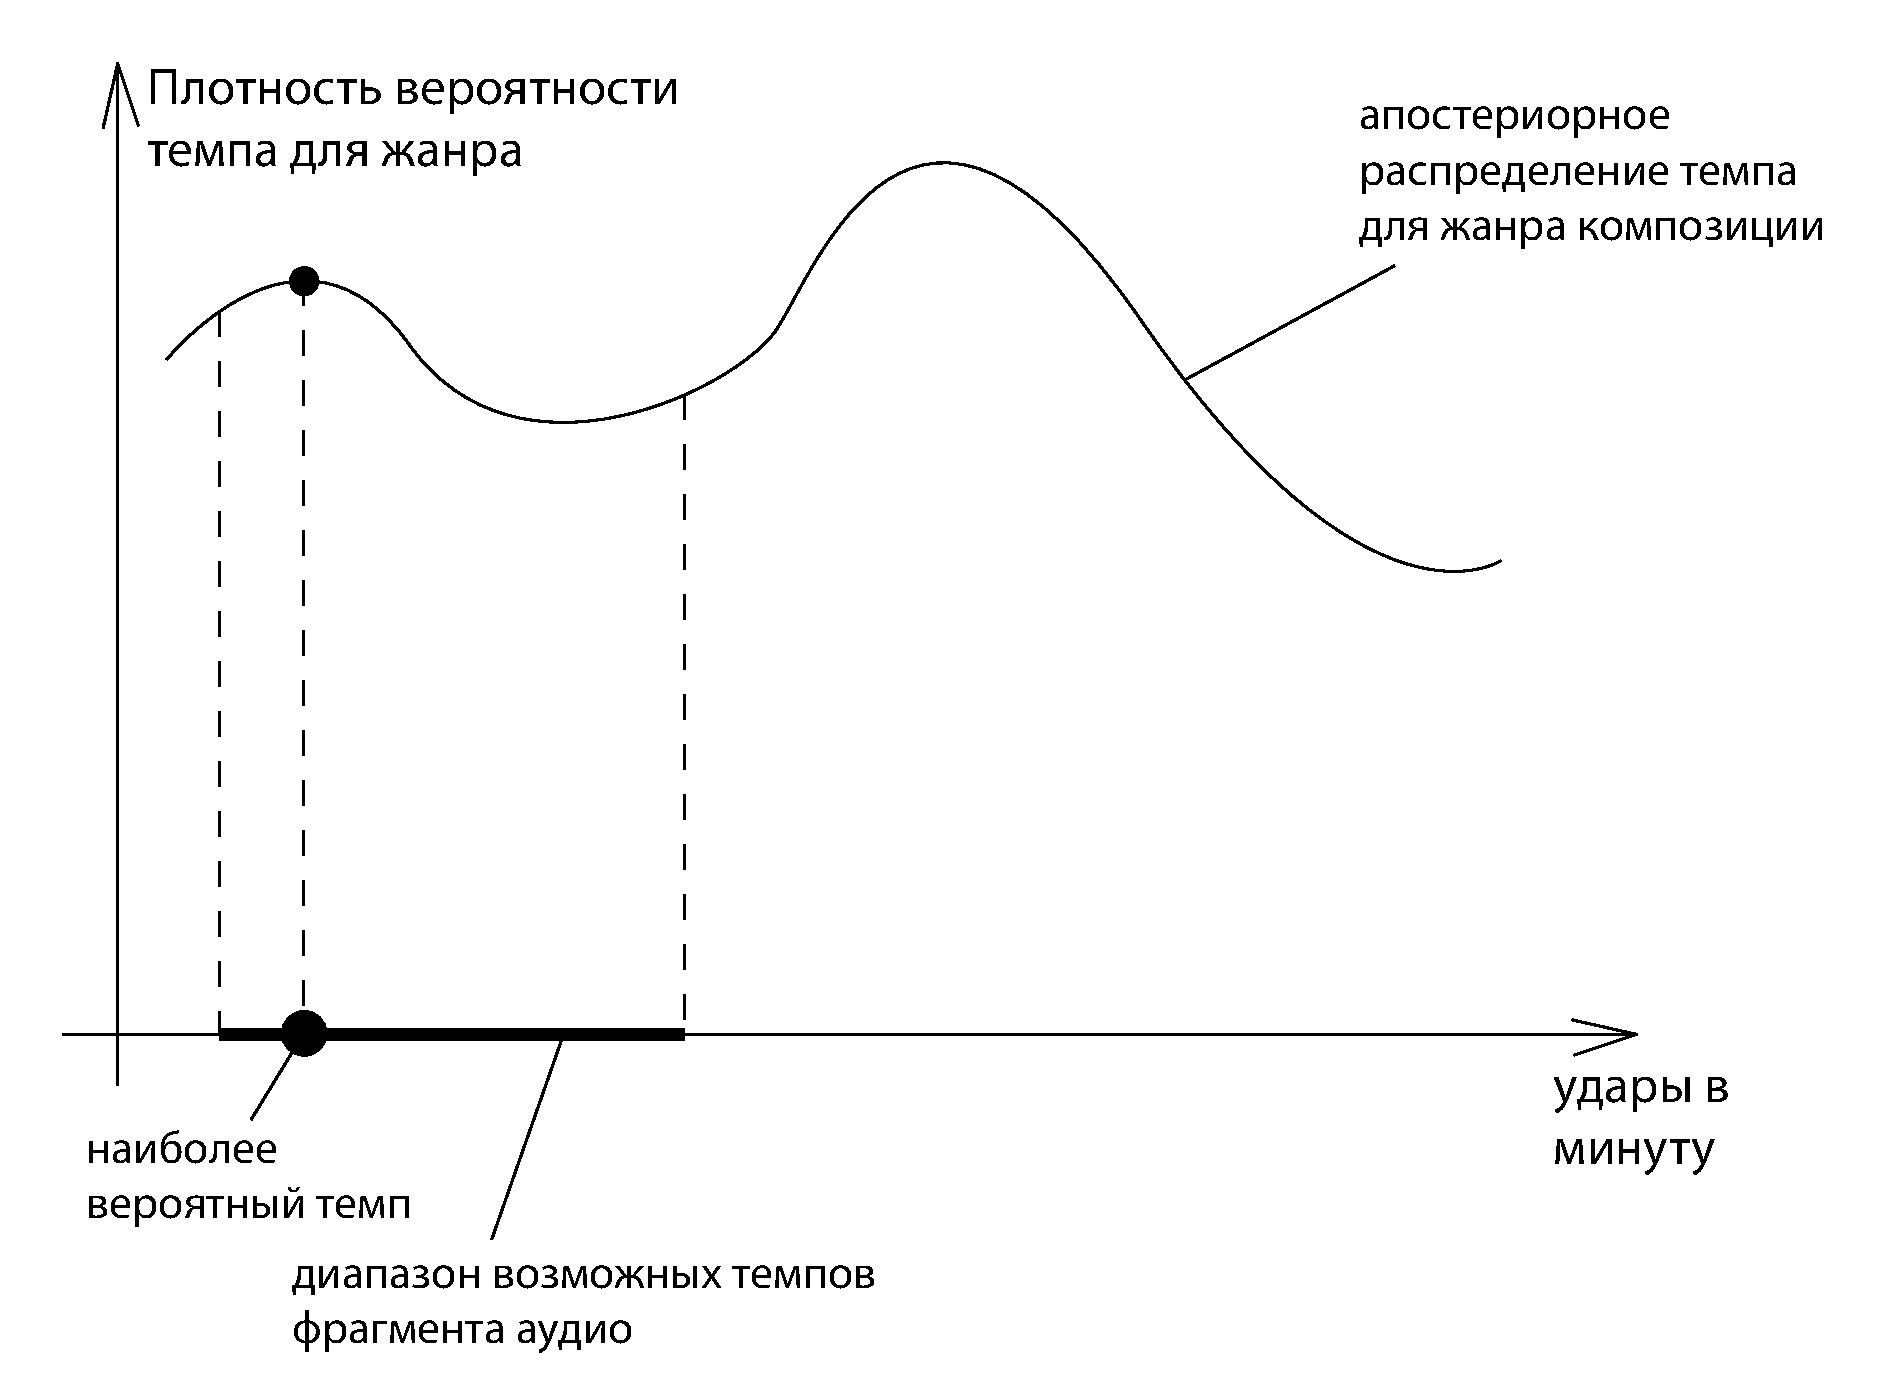
\includegraphics[scale=0.5]{svg/res_tempo.pdf}
	\caption{Нахождение наиболее вероятного темпа}
	\label{img:res_tempo}
\end{figure}

\clearpage

\subsection{Определение переменного ритма}

На рисунках \ref{img:rhythm_0} -- \ref{img:rhythm_3} приведены IDEF0-диаграммы для алгоритма определения переменного ритма (тактового размера) музыки.

\begin{figure}[h]
	\centering
	\includegraphics[scale=0.25]{inc/img/rhythm_idef/01_A-0.png}
	\caption{IDEF0 нулевого уровня}
	\label{img:rhythm_0}
\end{figure}

По аналогии с определением темпа в качестве априорного распределения тактового размера в байесовской модели выбрано равномерное распределение, так как на данном этапе, за неимением каких-либо других характеристик указанного аудиофайла, предполагается, что все размеры для него в заданных пределах равновероятны.

В качестве распределения функции правдоподобия размера выбрано нормальное распределение (поскольку распределение размеров в датасете также близко к нормальному) с математическим ожиданием, равным математическому ожиданию априорного, и дисперсией, также равной априорной.

\begin{figure}[h]
	\centering
	\includegraphics[scale=0.25]{inc/img/rhythm_idef/02_A0.png}
	\caption{Определение переменного ритма}
	\label{img:rhythm_1}
\end{figure}

\begin{figure}[h]
	\centering
	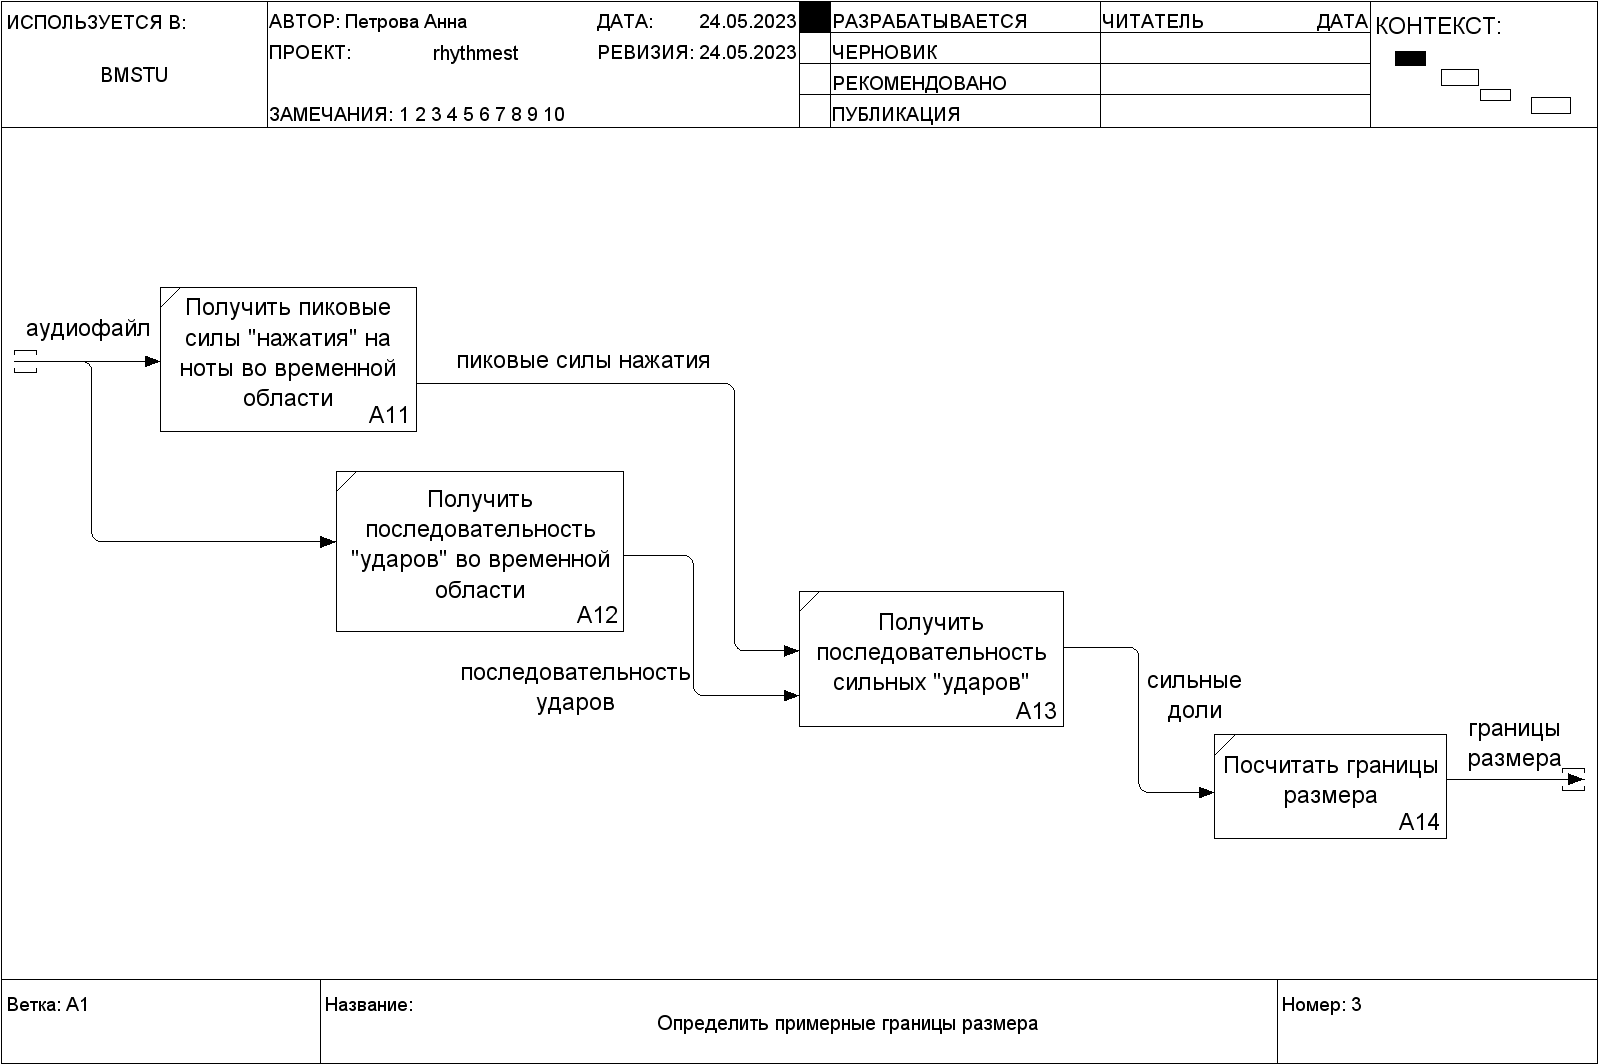
\includegraphics[scale=0.25]{inc/img/rhythm_idef/03_A1.png}
	\caption{Определение границ размера}
	\label{img:rhythm_2}
\end{figure}

\newpage

Для задания априорного распределения необходимо определить границы размера. Для этого во всем аудиофайле сначала находятся последовательности амплитуд и <<ударов>> во временной области. Последовательность <<ударов>> определяется на основе оценки темпа. В найденной последовательности амплитуд находятся пики (точки максимума). После чего пики амплитуд <<накладываются>> на последовательность <<ударов>> и получается последовательность сильных <<ударов>> (долей) (т.~е. предположительные начала тактов). Количество <<ударов>> между сильными долями и есть тактовый размер. Таким образом определяются примерные границы размеров рассматриваемого аудиофайла.

Остальное происходит аналогично определению темпа. Считается байесовская модель для оценки апостериорной вероятности размера. Далее аудиофайл разделяется на фрагменты по 5 секунд, для каждого фрагмента рассчитывается диапазон размеров по принципу, описанному выше. После чего полученное в результате моделирования апостериорное распределение размеров применяется к данному диапазону, и ищется максимум функции плотности, т.~е. наиболее вероятный тактовый размер фрагмента.

\begin{figure}[h]
	\centering
	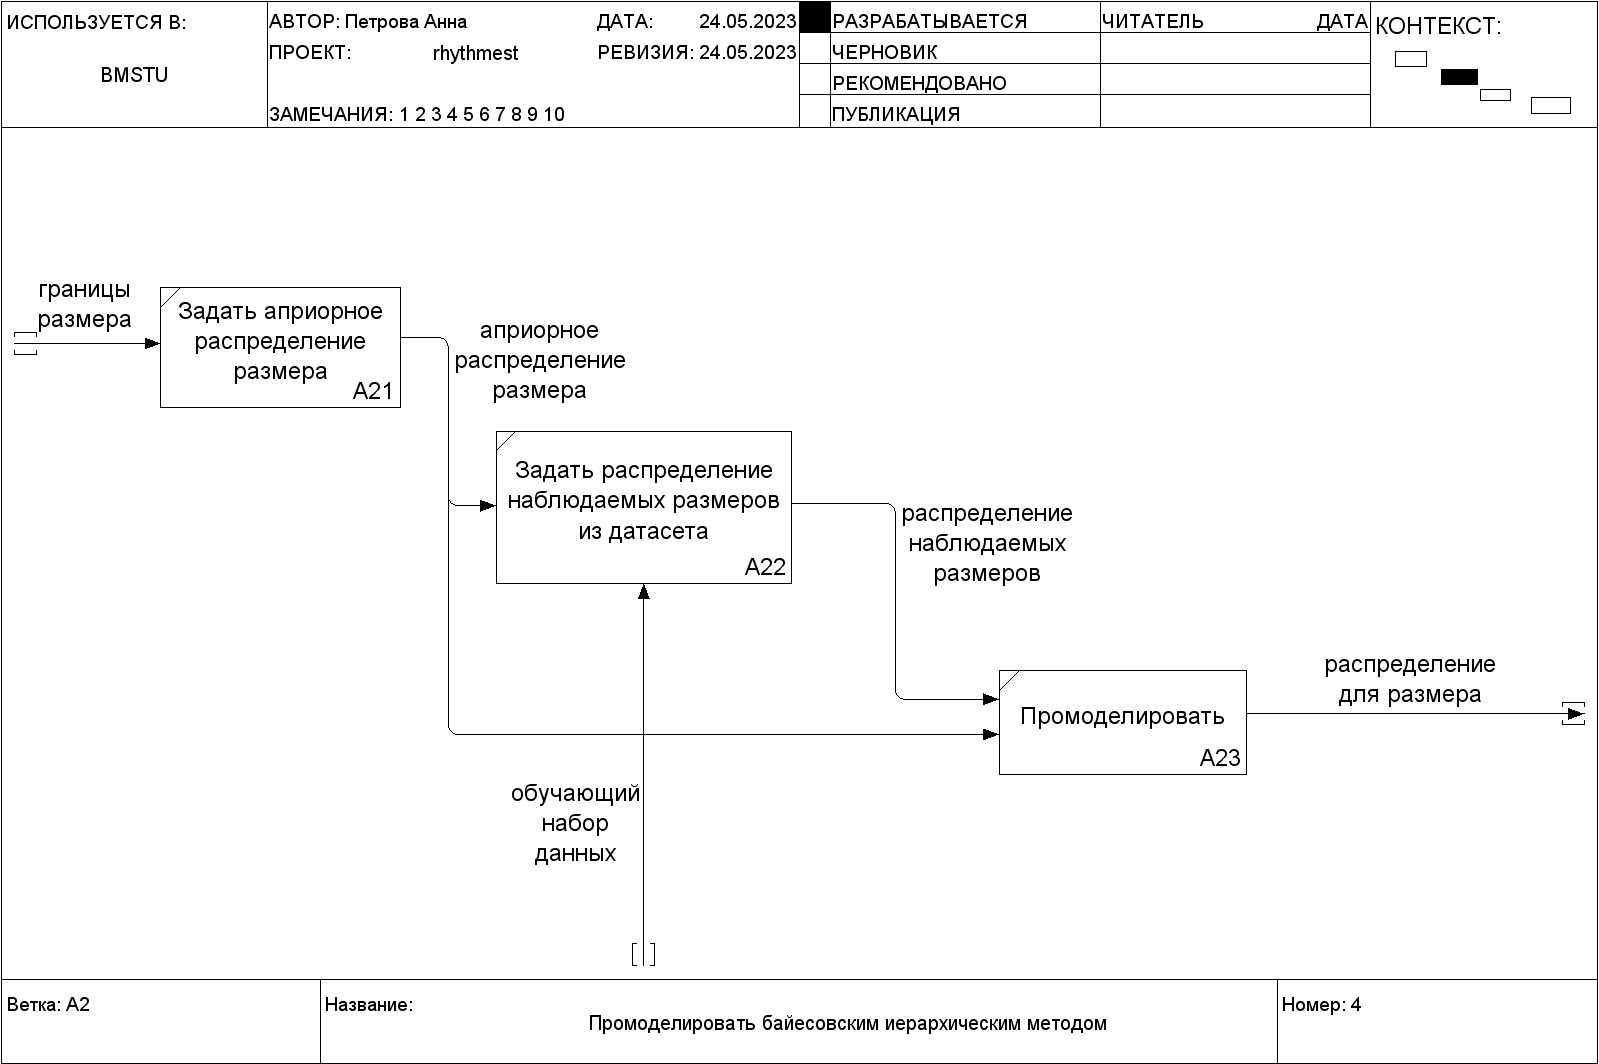
\includegraphics[scale=0.25]{inc/img/rhythm_idef/04_A2.png}
	\caption{Байесовское моделирование}
	\label{img:rhythm_3}
\end{figure}

\clearpage

\subsection{Структуры данных}

Результаты работы программы будут представлены в виде словарей, где в качестве ключей -- время от начала аудиофайла в секундах, а в качестве значений -- темпы или тактовые размеры соответственно.

Все распределения, значения из датасета, последовательности <<ударов>> и пики амплитуды будут представлены в виде списков. Списки <<ударов>> и пиков амплитуды представляют собой последовательность секунд от начала аудиозаписи, в которые происходят <<удары>> или пики амплитуды соответственно.

\subsection{Структура ПО}

На рисунке \ref{img:sw_structure} показана структура приложения, из которой видно, как происходит взаимодействие компонентов.

\begin{figure}[h]
	\centering
	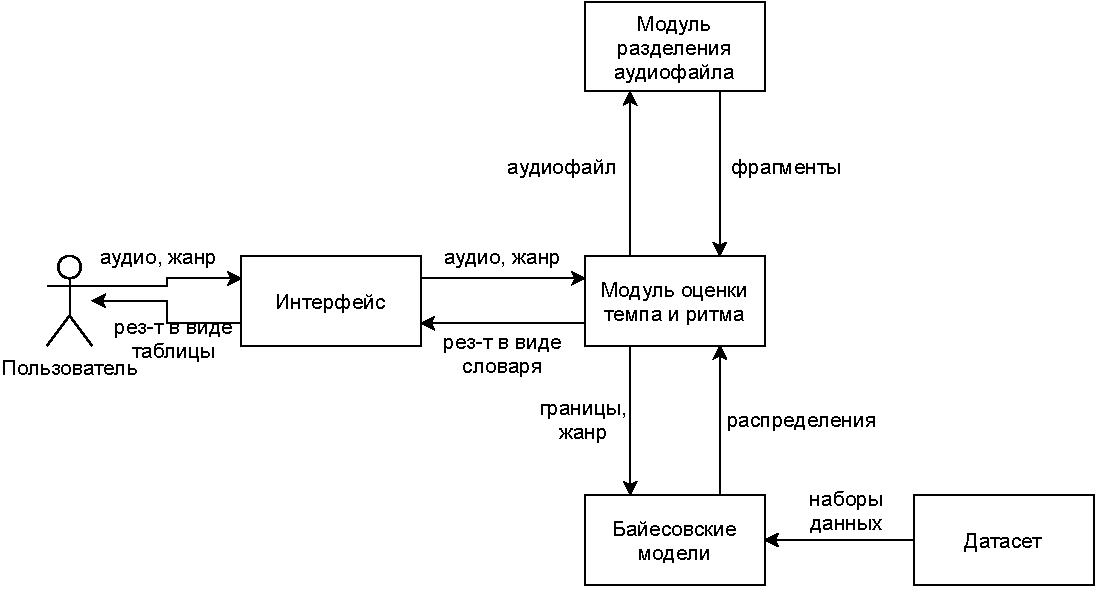
\includegraphics[scale=0.9]{svg/sw_structure.pdf}
	\caption{Структура приложения}
	\label{img:sw_structure}
\end{figure}

Модуль оценки темпа и ритма применяет результаты байесовского моделирования к фрагментам заданного аудиофайла.

\newpage

\subsection*{Выводы}

На основе теоретических данных, полученных в аналитическом разделе, был разработан метод определения переменного темпа и ритма музыки. Также были приведены IDEF0-диаграммы, схема структуры приложения и описаны основные структуры данных.


%\section{Технологический раздел}

\subsection{Выбор средств программной реализации}

В качестве языка программирования был выбран Python, так как:

\begin{itemize}
	\item[---] имеется достаточный опыт программирования на этом языке, что сократит время написания программы;
	\item[---] для данного языка программирования имеются все необходимые библиотеки для работы с байесовскими моделями и аудиофайлами, что также ускорит процесс разработки.
\end{itemize}

В качестве среды разработки был выбран PyCharm по следующим причинам:

\begin{itemize}
	\item[---] он бесплатен для использования студентами;
	\item[---] он имеет множество встроенных интсрументов, которые облегчают процесс написания и отладки кода;
	\item[---] имеется достаточный опыт программирования с использованием данной среды разработки, что сократит время изучения возможностей.
\end{itemize}

Для работы с аудиофайлами использовалась библиотека librosa~\cite{librosa}, а для реализации байесовских моделей -- библиотека PyMC3~\cite{pymc3_docs}. Кроме того в программе вместо обычных списков часто для удобства использовались numpy массивы~\cite{numpy}.

\subsection{Детали реализации}

\subsubsection{Байесовские модели}

В листингах \ref{lst:bpmmodel}, \ref{lst:measuremodel} представлена реализация байесовских иерархических моделей для оценки темпа и тактового размера соответственно.

\newpage

\begin{lstlisting}[label={lst:bpmmodel}, caption={реализация байесовской модели для определения темпа}]
	def bpm_model(min_bpm: int, max_bpm: int, bpm_dataset, genre_dataset, genres_ints, progress):
		with pm.Model() as model:
			# hyperpriors (lvl 1)
			tempo = pm.Uniform('tempo', lower=min_bpm, upper=max_bpm)
			progress.setValue(20)
			mu = (min_bpm + max_bpm) / 2.0
			sigma = (max_bpm - min_bpm) / 12.0
			genre_coef = pm.Normal('genre_coef', mu=0, sd=1, shape=len(genre_dataset.unique()))
			progress.setValue(40)
	
			# prior (lvl 2)
			bpm_est = mu + genre_coef[genres_ints] * sigma
			progress.setValue(60)
	
			# likelihood (lvl 3)
			bpm_obs = pm.Normal('bpm_obs', mu=bpm_est, sd=sigma, observed=bpm_dataset)
			progress.setValue(80)
	
			# get the samples
			trace = pm.sample(1000, tune=500, chains=2, cores=1)
			progress.setValue(100)
	
		return trace
\end{lstlisting}

\begin{lstlisting}[label={lst:measuremodel}, caption={реализация байесовской модели для определения ритма}]
	def rhythm_model(measure_min, measure_max, rhythm_dataset, progress):
		with pm.Model() as model:
			# prior
			measure = pm.Uniform('measure', lower=measure_min, upper=measure_max)
			progress.setValue(20)
			mu = (measure_min + measure_max) / 2.0
			progress.setValue(40)
			sigma = (measure_max - measure_min) / 12.0
			progress.setValue(60)
			# likelihood
\end{lstlisting}

\begin{lstlisting}
			measure_obs = pm.Normal('measure_obs', mu=mu, sd=sigma, observed=rhythm_dataset)
			progress.setValue(80)

			trace = pm.sample(1000, tune=1000, chains=2)
			progress.setValue(100)
	
		return trace
\end{lstlisting}

На вход моделей поступают границы темпа или размера, массив значений из датасета (для оценки темпа -- это темпы и жанры, для ритма -- размеры), список жанров, закодированных числами (для темпа) (для размещения коэффициентов по индексам жанров) и линия прогресса из интерфейса для ее обновления.

Выходными данными указанных функций являются распределения соответствующих параметров (в первом случае -- это темп и коэффициенты для всех жанров, а во втором -- тактовый размер).

Метод sample отвечает за сам процесс моделирования (получения апостериорных распределений).

Расчет диапазона возможных темпов был реализован с помощью метода beat\_track() из библиотеки librosa, в качестве дельты взято 40 bpm.

\subsubsection{Разделение аудиофайла}

В листинге \ref{lst:splitaudio} представлена реализация функции разделения аудиофайла на фрагменты.

\begin{lstlisting}[label={lst:splitaudio}, caption={разделение аудиофайла на фрагменты}]
	def split_mp3(audio_path: str, step: int):
		if not os.path.isdir("tmp"):
			os.mkdir("tmp")
		# load audio
		audio_file = AudioSegment.from_file(audio_path, format="mp3")
		# fragments length in milliseconds
		part_length = step
\end{lstlisting}

\begin{lstlisting}
		# split audio
		parts = [audio_file[i:i + part_length] for i in range(0, len(audio_file), part_length)]
		# save fragments
		for i, part in enumerate(parts):
			part.export(f"tmp/part_{i}.mp3", format="mp3")
\end{lstlisting}

Функция создает временную директорию <<tmp/>>, в которую впоследствии сохраняет фрагменты указанного аудиофайла в формате mp3. После расчета темпов или размеров для всех фрагментов созданная директория очищается и удаляется.

\subsubsection{Определение диапазона размеров}

В листинге~\ref{lst:measurerange} представлена реализация функций для расчета диапазона размеров.

\begin{lstlisting}[label={lst:measurerange}, caption={определение диапазона размеров}]
	def calc_measure(downbeats: list) -> int:
		downbeat_inds = [i for i, beat in enumerate(downbeats) if beat == 1]
		if len(downbeat_inds) <= 1:
			return 0
		difs_sum = 0
		for i in range(1, len(downbeat_inds)):
			difs_sum += (downbeat_inds[i] - downbeat_inds[i - 1])
		avg_measure = difs_sum / (len(downbeat_inds) - 1)
		return round(avg_measure)
	
	def get_measure_range(audio_path: str, tail: list):
		y, sr = librosa.load(audio_path)
		onset_env = librosa.onset.onset_strength(y=y, sr=sr)
		# amplitude peaks
		peaks = librosa.util.peak_pick(onset_env, pre_max=3, post_max=3, pre_avg=3,
		post_avg=5, delta=0.5, wait=10)
		peaks_time = librosa.frames_to_time(peaks, sr=sr)
		_, beats = librosa.beat.beat_track(onset_envelope=onset_env, sr=sr)
		beats_time = librosa.frames_to_time(beats, sr=sr)
\end{lstlisting}

\begin{lstlisting}
		# beginnings of bars
		downbeat_times = {}
		for i, beat in enumerate(beats_time):
		if beat in peaks_time:
		downbeat_times[i] = beat
		downbeats = [0 for i in range(len(beats))]
		for beat in downbeat_times.keys():
		downbeats[beat] = 1
		downbeats = tail + downbeats
		prior_measure = calc_measure(downbeats)
		if prior_measure == 0:
			return -1, downbeats
		if prior_measure > 2:
			return 0, np.arange(prior_measure - 2, prior_measure + 3, 1)
		elif prior_measure == 2:
			return 0, np.arange(prior_measure - 1, prior_measure + 3, 1)
		else:
			return 0, np.arange(prior_measure, prior_measure + 3, 1)
\end{lstlisting}

Функция calc\_measure отвечает за расчет тактового размера на основе списка из чередующихся сильных и слабых долей, где сильные доли обозначаются 1, а слабые -- 0.

Если в указанном отрывке найдена только одна сильная доля, то этот фрагмент объединяется со следующим. Для этого среди входных данных функции get\_measure\_range есть параметр tail, который представляет собой список сильных и слабых долей предыдущего фрагмента аудио.

Набор сильных долей формируется на основе совпадений времени в двух списках: пиков амплитуды (peaks\_time) и <<ударов>> (beats\_time).

\subsection{Пользовательский интерфейс}

На рисунке~\ref{img:gui} представлен интерфейс разработанного приложения.

Приложение поддерживает загрузку только mp3 файлов. Список возможных жанров загружаемой музыки был создан на основе датасета. Темпы и размеры можно определять отдельно, независимо друг от друга.

\begin{figure}[h]
	\centering
	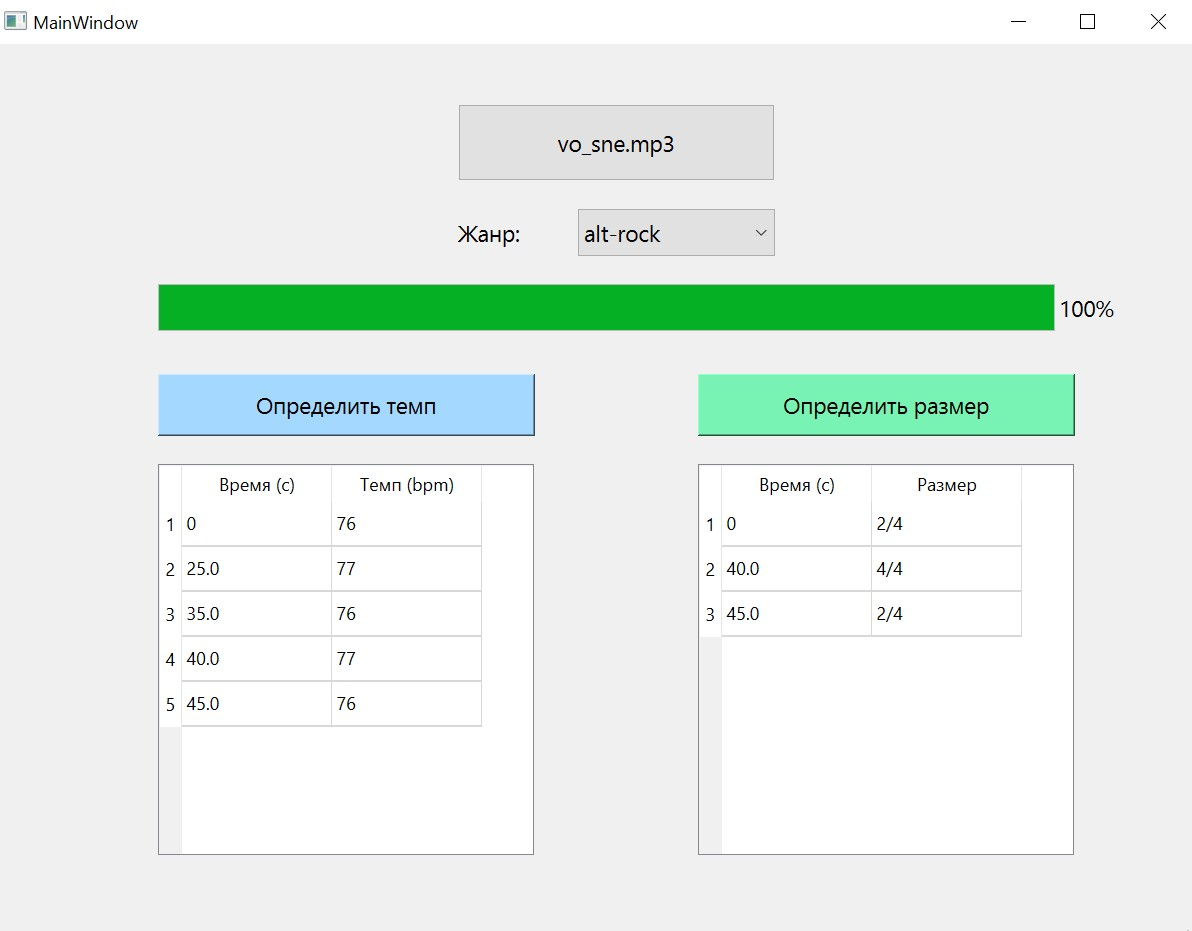
\includegraphics[scale=0.7]{inc/img/gui.jpg}
	\caption{Интерфейс приложения}
	\label{img:gui}
\end{figure}

Для того, чтобы определить темп аудиофайла, необходимо:

\begin{enumerate}
	\item Загрузить аудиофайл, нажав на верхнюю кнопку.
	\item Выбрать жанр загруженной музыки из выпадающего списка ниже.
	\item Нажать на кнопку <<Определить темп>>.
	\item Результаты появятся в левой таблице через 1,5-2 минуты.
\end{enumerate}

Для определения ритма:

\begin{enumerate}
	\item Загрузить аудиофайл, нажав на верхнюю кнопку.
	\item Нажать на кнопку <<Определить размер>>.
	\item Результаты появятся в правой таблице в течение минуты.
\end{enumerate}

Жанр в этом случае указывать необязательно.

\newpage

\subsection{Тестирование приложения}

В процессе разработки приложения проводились модульные тесты (листинг~\ref{lst:units}). Тестировались такие функции, как: разделение аудиофайла на фрагменты, очистка директории, удаление директории и расчет тактового размера на основе списка сильных и слабых долей.

\begin{lstlisting}[label={lst:units}, caption={модульные тесты}]
	class SplitAudio(unittest.TestCase):
		def test_splitting(self):
			audio = "test_audio/vo_sne.mp3"
			step = 5000
			split_mp3(audio, step)
			self.assertEqual(os.path.exists("tmp/"), True)
			self.assertGreater(len(os.listdir("tmp/")), 0)
	
	class CleanDirs(unittest.TestCase):
		def test_cleaning(self):
			os.mkdir("temp/")
			fp = open('temp/file.txt', 'x')
			fp.close()
			dir = "temp/"
			clean_dir(dir)
			self.assertEqual(len(os.listdir(dir)), 0)
			os.rmdir(dir)
		def test_removing(self):
			os.mkdir("temp/")
			dir = "temp/"
			remove_dir(dir)
			self.assertEqual(os.path.exists("temp/"), False)
	
	class CalcMeasure(unittest.TestCase):
		def test_calculating(self):
			downbeats = [1, 0, 0, 0, 1, 0, 0, 0, 1]
			measure = calc_measure(downbeats)
			self.assertEqual(measure, 4)
\end{lstlisting}

Как видно из рисунка~\ref{img:units}, все модульные тесты были успешно пройдены.

\begin{figure}[h]
	\centering
	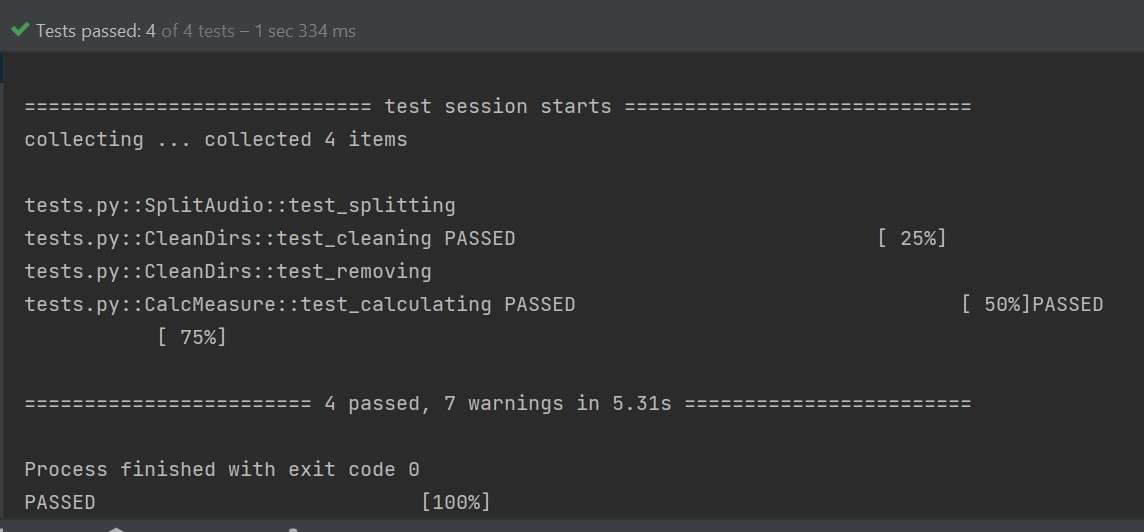
\includegraphics[scale=0.8]{inc/img/units.jpg}
	\caption{Результаты модульного тестирования}
	\label{img:units}
\end{figure}

\newpage

Работоспособность программы в целом проверялась вручную. На рисунке~\ref{img:test_const} представлены результаты работы программы на одном из аудиофайлов.

\begin{figure}[h]
	\centering
	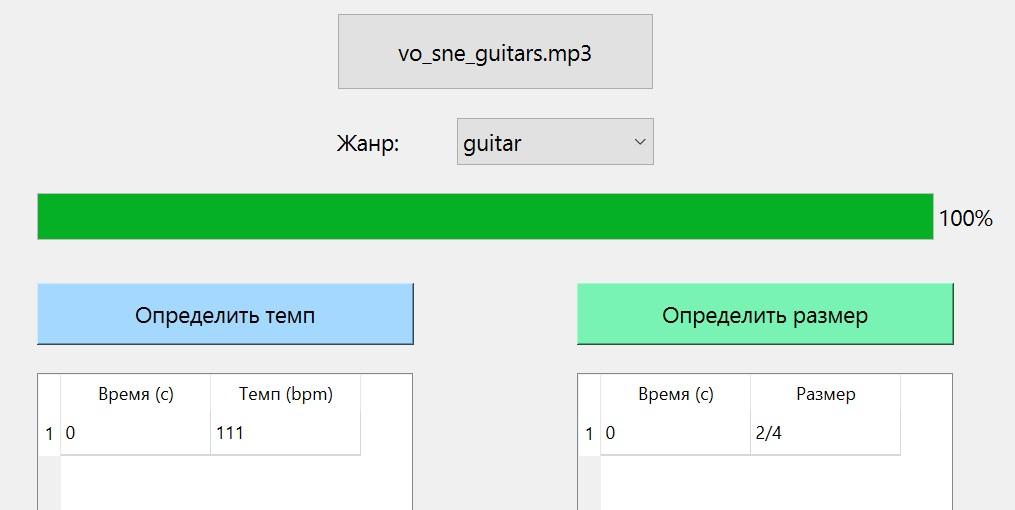
\includegraphics[scale=0.9]{inc/img/test_constant.jpg}
	\caption{Результаты для постоянного темпа и ритма}
	\label{img:test_const}
\end{figure}

\newpage

При этом заранее известно, что темп данной аудиозаписи 125 bpm, а тактовый размер -- 4/4 (рис.~\ref{img:vosne_ref}, самое левое число -- темп в bpm, правее -- размер).

\begin{figure}[h]
	\centering
	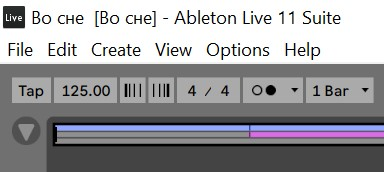
\includegraphics[scale=1.4]{inc/img/vosne_ref.jpg}
	\caption{Эталонные значения темпа и размера}
	\label{img:vosne_ref}
\end{figure}

Таким образом, отклонение полученного темпа от идеального составляет примерно 11\%, что является приемлемым результатом, поскольку согласно исследованиям~\cite{bayesian} ошибки байесовского метода могут составлять до 18\%.

Размер 2/4 также является допустимым результатом в данном случае. Это означает, что сильных долей в аудиозаписи было выявлено в два раза больше, но при этом основной ритм остается тем же, что и при 4/4 (т.~к. два такта по 2/4 дают в сумме один такт с размером 4/4).

Для тестирования определения переменного темпа использовался аудиофайл с темпом 115 bpm в первые 25 секунд и 120 bpm в оставшееся время (размер этого музыкального фрагмента постоянен и равен 6/8, что в данном случае может быть приравнено к 3/4).

Результаты работы метода представлены на рисунке~\ref{img:test_tempo}.

Ошибка определения темпа в данном случае составляет примерно 7\%, что также укладывается в допустимые пределы.

Для тестирования определения переменного ритма использовался аудиофайл с размером 3/4 в первые 15 секунд и 4/4 bpm в оставшееся время (темп этого музыкального фрагмента постоянен и равен 100 bpm).

Результаты работы метода представлены на рисунке~\ref{img:test_rhythm}.

Ошибка определения размера в таком случае составляет примерно 8\%.

\begin{figure}[h]
	\centering
	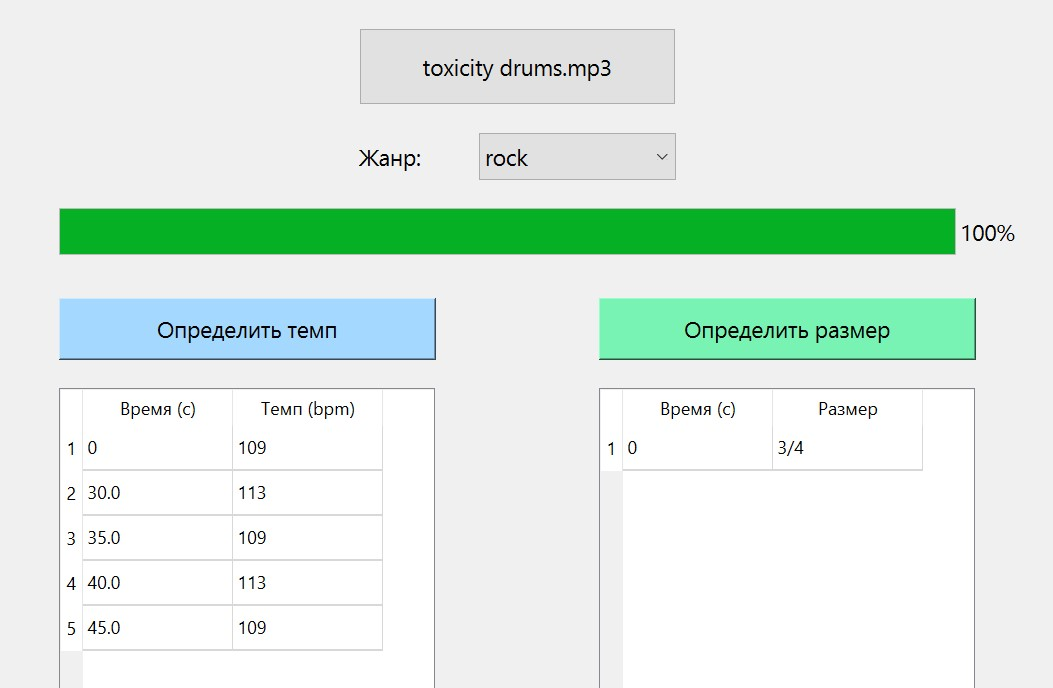
\includegraphics[scale=0.85]{inc/img/test_tempo.jpg}
	\caption{Результаты для переменного темпа}
	\label{img:test_tempo}
\end{figure}

\begin{figure}[h]
	\centering
	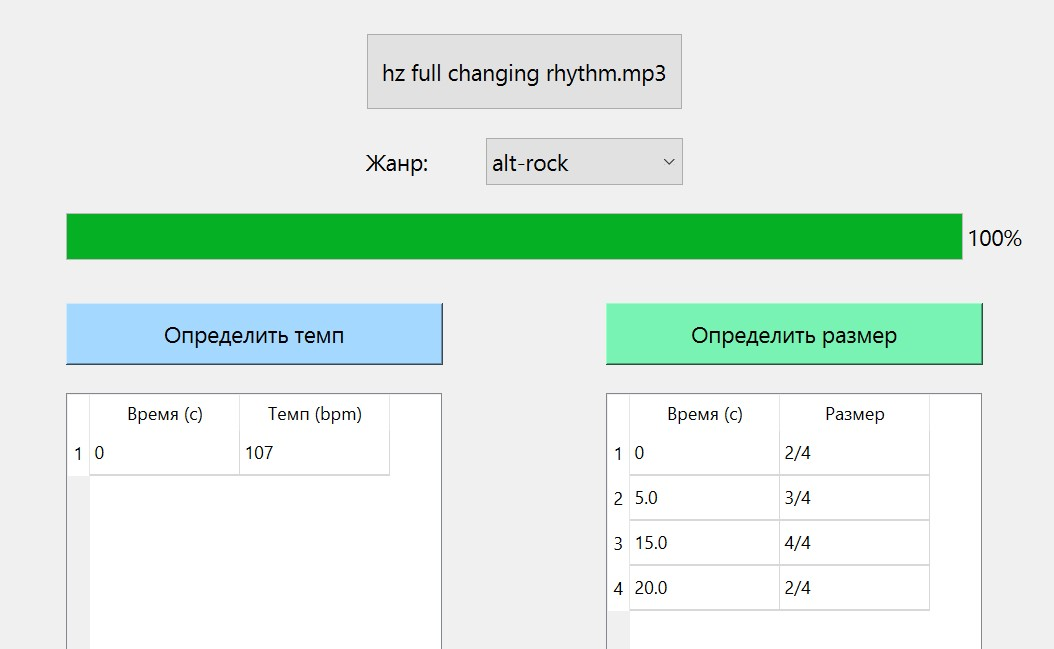
\includegraphics[scale=0.85]{inc/img/test_rhythm.jpg}
	\caption{Результаты для переменного размера}
	\label{img:test_rhythm}
\end{figure}

\clearpage

\subsection*{Выводы}

В данном разделе были выбраны язык программирования и среда разработки, а также приведены детали реализации, пользовательский интерфейс и результаты тестирования разработанной программы.

В качестве языка программирования был выбран Python, а в качестве среды разработки -- PyCharm.

Была описана реализация байесовских моделей для определения ритма и темпа, разделения аудиофайла на фрагменты и определения диапазона размеров.

Все модульные тесты были успешно пройдены. Результаты функциональных тестов также оказались в пределах допустимости.

%\section{Исследовательский раздел}
\setcounter{figure}{0}
\setcounter{table}{0}
\subsection{Сравнение результатов работы метода с существующим аналогом}

Сравнение результатов работы метода по определению темпа музыки производилось с результатами работы метода beat\_track() из библиотеки librosa. Этот метод определяет средний темп для указанного аудиофайла, поэтому для сравнения аудиозапись также разделялась на 5-секундные фрагменты, для каждой из которых вызывался этот метод.

Исследование проводилось на 8 аудиофайлах с переменным темпом и на 8 с постоянным. Все аудиофайлы были сгруппированы по жанрам. Таким образом, в случае с переменным темпом использовались музыкальные композиции в поп, рок и соул жанрах, а в случае с постоянным темпом -- в фанк, джаз, поп и рок жанрах.

На рисунках~\ref{img:tempo_librosa_change} -- \ref{img:tempo_librosa_const} представлены гистограммы, отображающие точность оценки переменного и постоянного темпа исследуемых программных решений.

Как видно из гистограмм, разработанный метод превосходит библиотеку в точности оценки переменного темпа музыки, но при этом в точности определения постоянного темпа в большинстве случаев уступает аналогу.

\begin{figure}[h]
	\centering
	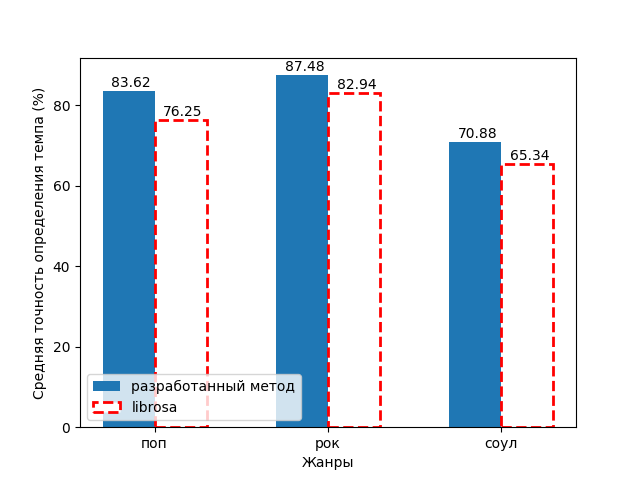
\includegraphics[scale=0.9]{../graphs/changing_tempo_librosa.png}
	\caption{Точность результатов работы ПО и аналога при переменном темпе}
	\label{img:tempo_librosa_change}
\end{figure}

\begin{figure}[h]
	\centering
	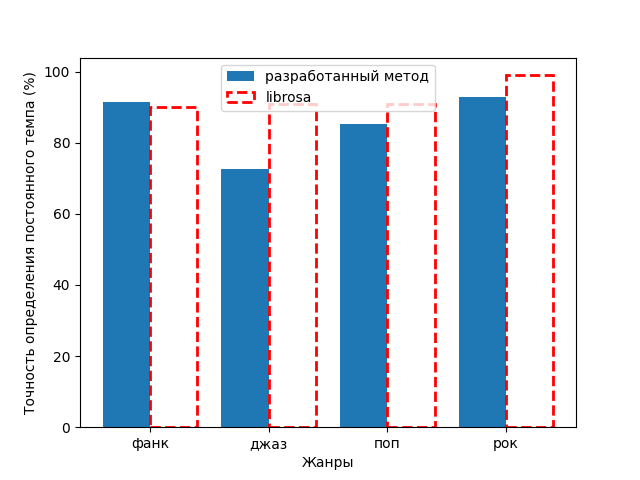
\includegraphics[scale=0.9]{../graphs/const_tempo_librosa.png}
	\caption{Точность результатов работы ПО и аналога при постоянном темпе}
	\label{img:tempo_librosa_const}
\end{figure}
\clearpage
\subsection{Применимость ПО для аудиозаписей с разным набором инструментов}

В качестве тестовых данных для анализа ритма использовались аудиофайлы со следующими инструментами:
 
\begin{enumerate}
	\item Только ударные.
	\item Только гитара.
	\item Гитара вместе с ударными.
\end{enumerate}

Во всех трех аудиозаписях использовался один и тот же музыкальный фрагмент с переменным размером (3/4 первые 15 секунд и 4/4 оставшееся время) (см. рис.~\ref{img:hz_ref}).

\begin{figure}[h]
	\centering
	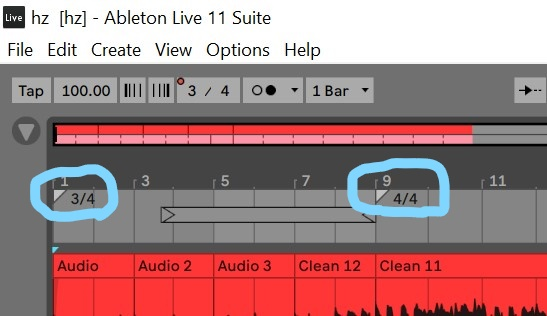
\includegraphics[scale=0.7]{inc/img/hz_ref.jpg}
	\caption{Эталонные значения размера}
	\label{img:hz_ref}
\end{figure}

%\newpage

Результаты работы ПО по определению переменного размера для трех указанных аудиофайлов представлены в таблицах~\ref{tab:hz_drums} -- \ref{tab:hz_full} соответственно.

\begin{table}[!h]
	\begin{center}
		\caption{\label{tab:hz_drums}Результаты для 1-го аудиофайла}
		\begin{tabular}{|p{8cm}|p{8cm}|}
			\hline
			Время (с) & Размер\\
			\hline
			0 & 3/4\\
			\hline
			15 & 4/4\\
			\hline
		\end{tabular}
	\end{center}
\end{table}

\begin{table}[!h]
	\begin{center}
		\caption{\label{tab:hz_guitar}Результаты для 2-го аудиофайла}
		\begin{tabular}{|p{8cm}|p{8cm}|}
			\hline
			Время (с) & Размер\\
			\hline
			0 & 2/4\\
			\hline
			5 & 3/4\\
			\hline
			10 & 2/4\\
			\hline
			20 & 1/4\\
			\hline
		\end{tabular}
	\end{center}
\end{table}

\begin{table}[!h]
	\begin{center}
		\caption{\label{tab:hz_full}Результаты для 3-го аудиофайла}
		\begin{tabular}{|p{8cm}|p{8cm}|}
			\hline
			Время (с) & Размер\\
			\hline
			0 & 2/4\\
			\hline
			5 & 3/4\\
			\hline
			15 & 4/4\\
			\hline
			20 & 2/4\\
			\hline
		\end{tabular}
	\end{center}
\end{table}

\newpage

На рисунке~\ref{img:measure_instr} приведена средняя точность оценки тактового размера (в процентах) в зависимости от набора инструментов в аудиозаписи.

\begin{figure}[h]
	\centering
	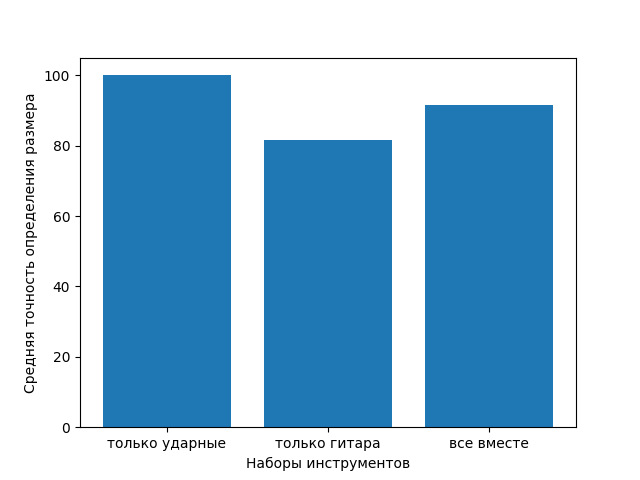
\includegraphics[scale=0.89]{../graphs/measure_instr.png}
	\caption{точность оценки размера в зависимости от инструментов}
	\label{img:measure_instr}
\end{figure}

\newpage

Как видно из гистограммы, наибольшую точность программа выдает на аудиофайле с ударными, а наименьшую -- на аудиозаписи с гитарой. Такие результаты могут быть связаны с небольшими отклонениями гитары от ритмической сетки, а также со смещением сильных долей в гитарной партии. При этом во всех случаях точность определения тактового размера лежит в допустимых пределах ($\ge82\%$).

Для анализа темпа в свою очередь использовались аудиофайлы со следующими инструментами:

\begin{enumerate}
	\item Только ударные.
	\item Гитары и бас.
	\item Ударные, бас и гитара.
	\item Полный фрагмент (ударные, бас, гитара и вокал).
\end{enumerate}

Здесь использовался другой музыкальный фрагмент, также одинаковый для всех трех аудиофайлов, с переменным темпом (115 bpm первые 25 секунд и 120 bpm оставшееся время) (<<Toxicity>> - System of a down).

Результаты работы ПО по определению переменного темпа для этих аудиофайлов представлены в таблицах~\ref{tab:soad_drums} -- \ref{tab:soad_full} соответственно.

\begin{table}[!h]
	\begin{center}
		\caption{\label{tab:soad_drums}Результаты для 1-го аудиофайла}
		\begin{tabular}{|p{8cm}|p{8cm}|}
			\hline
			Время (с) & Темп (bpm)\\
			\hline
			0 & 105\\
			\hline
			30 & 113\\
			\hline
			35 & 105\\
			\hline
			40 & 113\\
			\hline
			45 & 105\\
			\hline
		\end{tabular}
	\end{center}
\end{table}

\begin{table}[!h]
	\begin{center}
		\caption{\label{tab:soad_guitar}Результаты для 2-го аудиофайла}
		\begin{tabular}{|p{8cm}|p{8cm}|}
			\hline
			Время (с) & Темп (bpm)\\
			\hline
			0 & 91\\
			\hline
			30 & 186\\
			\hline
			35 & 91\\
			\hline
			40 & 160\\
			\hline
			45 & 91\\
			\hline
		\end{tabular}
	\end{center}
\end{table}

\begin{table}[!h]
	\begin{center}
		\caption{\label{tab:soad_minus}Результаты для 3-го аудиофайла}
		\begin{tabular}{|p{8cm}|p{8cm}|}
			\hline
			Время (с) & Темп (bpm)\\
			\hline
			0 & 131\\
			\hline
			5 & 103\\
			\hline
			10 & 131\\
			\hline
			15 & 103\\
			\hline
			20 & 131\\
			\hline
		\end{tabular}
	\end{center}
\end{table}

\begin{table}[!h]
	\begin{center}
		\caption{\label{tab:soad_full}Результаты для 4-го аудиофайла}
		\begin{tabular}{|p{8cm}|p{8cm}|}
			\hline
			Время (с) & Темп (bpm)\\
			\hline
			0 & 103\\
			\hline
			5 & 93\\
			\hline
			10 & 103\\
			\hline
			15 & 93\\
			\hline
		\end{tabular}
	\end{center}
\end{table}

\newpage

На рисунке~\ref{img:tempo_instr} приведена средняя точность оценки темпа в зависимости от набора инструментов в аудиозаписях для разработанного ПО.

\begin{figure}[h]
	\centering
	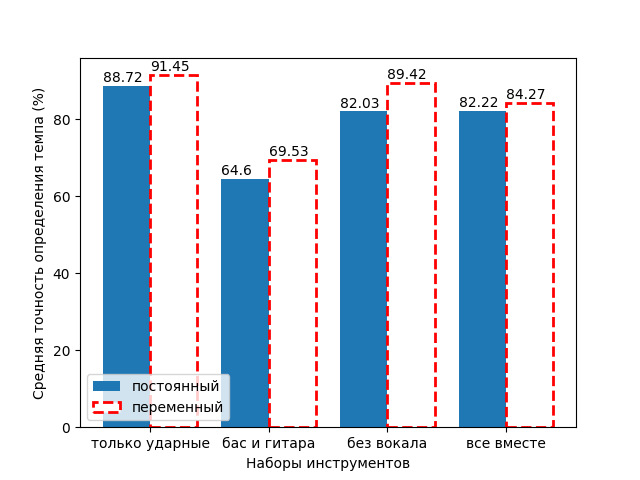
\includegraphics[scale=1]{../graphs/tempo_instr.png}
	\caption{точность оценки темпа в зависимости от инструментов}
	\label{img:tempo_instr}
\end{figure}

%\newpage

Как видно из гистограммы, наилучшие результаты разработанная программа показывает на аудизаписи, содержащей только ударные, и на аудиозаписи без вокала (с ударными, басом и гитарой). Наименьшая точность результатов получилась на аудиофайле, содержащем только гитару и бас. Помимо перечисленных ранее причин, это может быть связано также с проблемами в качестве этой записи.

\newpage

\subsection{Применимость ПО для музыки разных жанров}

Для исследования работы ПО в данном случае использовались следующие жанры:

\begin{itemize}
	\item[---] поп;
	\item[---] рок;
	\item[---] фанк;
	\item[---] джаз.
\end{itemize}

Примеры результатов работы метода по определению темпа для перечисленных жанров представлены в таблицах~\ref{tab:tempo_genres} -- \ref{tab:tempo_jazz}.

\begin{table}[!h]
	\begin{center}
		\caption{\label{tab:tempo_genres}Результаты определения темпа для разных жанров}
		\begin{tabular}{|p{8cm}|p{8cm}|}
			\hline
			\textbf{Жанр} & \textbf{Темп (bpm)}\\
			\hline
			Поп & 118\\
			\hline
			Рок & 113\\
			\hline
			Фанк & 119\\
			\hline
		\end{tabular}
	\end{center}
\end{table}

\begin{table}[!h]
	\begin{center}
		\caption{\label{tab:tempo_jazz}Результаты определения темпа для джаза}
		\begin{tabular}{|p{8cm}|p{8cm}|}
			\hline
			\textbf{Время (с)} & \textbf{Темп (bpm)}\\
			\hline
			0 & 85\\
			\hline
			5 & 99\\
			\hline
			30 & 85\\
			\hline
			35 & 99\\
			\hline
			60 & 128\\
			\hline
			65 & 99\\
			\hline
			80 & 128\\
			\hline
			85 & 191\\
			\hline
			90 & 87\\
			\hline
			95 & 33\\
			\hline
			100 & 99\\
			\hline
			115 & 191\\
			\hline
			120 & 99\\
			\hline
		\end{tabular}
	\end{center}
\end{table}

\newpage

Для расчета точности был собран и размечен датасет по 3-5 аудиофайлов для каждого жанра (как для постоянного темпа или ритма, так и для переменного).

\newpage

На рисунке~\ref{img:tempo_genres} представлена точность определения темпа музыки в зависимости от жанра.

\begin{figure}[h]
	\centering
	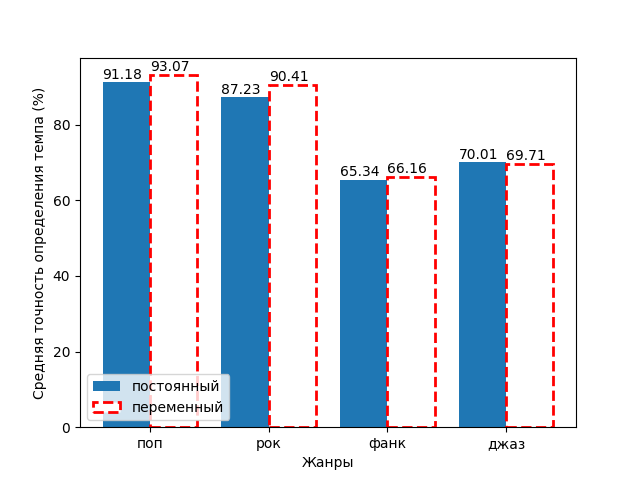
\includegraphics[scale=1]{../graphs/tempo_genres.png}
	\caption{точность оценки темпа в зависимости от жанра}
	\label{img:tempo_genres}
\end{figure}

Пример результатов по определению ритма для тех же жанров приведен в таблице~\ref{tab:rhythm_genres}.

\begin{table}[!h]
	\begin{center}
		\caption{\label{tab:rhythm_genres}Результаты определения ритма для разных жанров}
		\begin{tabular}{|p{8cm}|p{8cm}|}
			\hline
			\textbf{Жанр} & \textbf{Ритм}\\
			\hline
			Поп & 2/4\\
			\hline
			Рок & 2/4\\
			\hline
			Фанк & 5/4\\
			\hline
			Джаз & 3/4\\
			\hline
		\end{tabular}
	\end{center}
\end{table}

\newpage

На рисунке~\ref{img:measure_genres} представлена точность определения тактового размера в зависимости от жанра.

\begin{figure}[h]
	\centering
	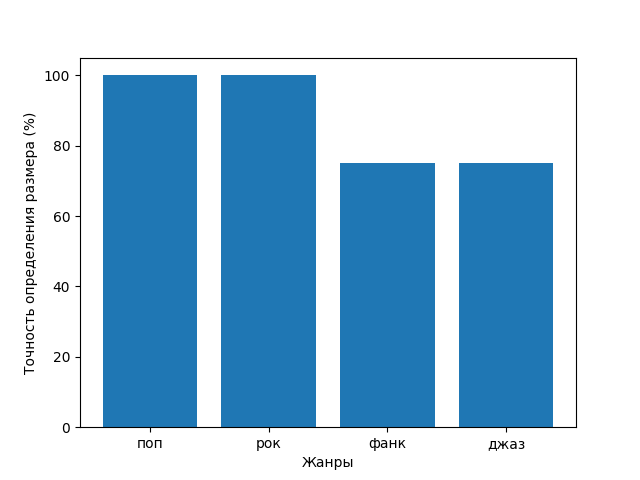
\includegraphics[scale=1]{../graphs/measure_genres.png}
	\caption{точность оценки размера в зависимости от жанра}
	\label{img:measure_genres}
\end{figure}

Как видно из гистограмм, точность оценки темпа и ритма значительно снижается на таких жанрах, как фанк и джаз. Это связано с особенностями этих жанров, такими как смещение ритма и сильных долей, что в свою очередь влияет и на определение темпа.

\subsection{Оценка разработанного метода}

В результате исследований у разработанного метода были выявлены следующие достоинства:

\begin{itemize}
	\item[---] более точное определение переменного темпа в сравнении с библиотечным методом;
	\item[---] высокая точность определения темпа и ритма для аудиозаписей с ударными;
	\item[---] высокая точность определения темпа и ритма для рок и поп музыки.
\end{itemize}

При этом у метода были обнаружены такие недостатки, как:

\begin{itemize}
	\item[---] менее точное определение постоянного темпа по сравнению с библиотечным методом;
	\item[---] более существенные ошибки при оценке темпа и ритма музыки, содержащей только гитары;
	\item[---] большие ошибки при определении тактового размера и темпа музыки таких жанров, как фанк и джаз.
\end{itemize}

\subsection*{Выводы}
В данном разделе был проведён анализ применимости разработанного метода для музыки с разным составом инструментов и разных жанров. 

В результате было выяснено, что наиболее высокой точности определения темпа и ритма метод достигает на музыке, содержащей ударные инструменты, а также в рок и поп жанрах.

Помимо этого, было проведено сравнение результатов разработанного метода с результатами библиотечной функции для определения темпа и выяснено, что разработанный метод превосходит библиотечный в точности при оценке переменного темпа примерно на 15\%.
\specsection{Заключение}

В результате работы были рассмотрены понятия предметной области, такие как темп и ритм музыки, и проанализирована проблема автоматического определения темпа и ритма.

Были определены критерии сравнения методов.

Были рассмотрены основные методы автоматического определения темпа и ритма музыки: дискретное вейвлет-преобразование, скрытые марковские модели, байесовское иерархическое моделирование и сверточные нейронные сети. После чего было произведено сравнение изученных методов по выделенным ранее критериям.

Таким образом, цель работы -- изучить основные существующие методы определения ритмического рисунка и темпа цифровой музыкальной записи -- была достигнута.

% говно литература для тест ВКР
\specsection{СПИСОК ИСПОЛЬЗОВАННЫХ ИСТОЧНИКОВ}

\begingroup
\renewcommand{\section}[2]{}
\begin{thebibliography}{}
	
\bibitem{dataset}
Spotify Tracks Dataset [Электронный ресурс]. -- Режим доступа: https://www.kaggle.com/datasets/maharshipandya/-spotify-tracks-dataset (15.05.2023).

\bibitem{kubler_pymc3}
Kübler R. Bayesian Hierarchical Modeling in PyMC3. -- 2021.

\bibitem{bayesian}
Nakamura E., Itoyama K., Yoshii K. Rhythm transcription of MIDI performances based on Hierarchical Bayesian Modelling of repetition and modification of musical note patterns. -- 2016.

\bibitem{pymc3_docs}
PyMC3 Documentation [Электронный ресурс]. -- Режим доступа: \url{https://www.pymc.io/projects/docs/en/v3/} (дата обращения: 17.05.2023).

\bibitem{librosa}
Librosa: audio and music processing in Python [Электронный ресурс]. -- Режим доступа: \url{https://librosa.org/doc/latest/index.html} (дата обращения: 17.05.2023).

\bibitem{pyqt}
PyQt Documentation v6.5.0 [Электронный ресурс]. -- Режим доступа: \url{https://www.riverbankcomputing.com/static/Docs/PyQt6/} (дата обращения: 20.05.2023).

\end{thebibliography}
\endgroup

% норм по феншую
%\bibliographystyle{utf8gost705u}
%\renewcommand{\refname}{СПИСОК ИСПОЛЬЗОВАННЫХ ИСТОЧНИКОВ}
%\bibliography{bibliography}

\anonsection{ПРИЛОЖЕНИЕ А}

\begin{lstlisting}[caption={модуль оценки темпа и ритма}]
	import pandas as pd
	import librosa
	from scipy import stats
	import numpy as np
	import os
	
	def genres_to_ints(genre_dataset):
		all_genres = genre_dataset.unique()
		genres_dict = {}
		for i, genre in enumerate(all_genres):
			genres_dict[genre] = i
		genres_ints = np.array([0] * len(genre_dataset))
		for i, genre in enumerate(genre_dataset.values):
			genres_ints[i] = genres_dict[genre]
		return genres_ints
	
	def get_tempo_bounds(bpm_dataset, genre_dataset, track_genre: str):
		rows_num = [i for i in range(len(genre_dataset)) if genre_dataset.values[i] == track_genre]
		tempos = [bpm_dataset.values[i] for i in rows_num]
		max_bpm = max(tempos)
		min_bpm = min(tempos)
		return min_bpm, max_bpm
	
	def estimate_bpm(audio_path: str, bpm_dataset, genre_dataset, track_genre: str, step: int, progress) -> dict:
		y, sr = librosa.load(audio_path)
		prior_bpm, _ = librosa.beat.beat_track(y=y, sr=sr)
		print(prior_bpm)
		min_bpm, max_bpm = get_tempo_bounds(bpm_dataset, genre_dataset, track_genre)
		genres_ints = genres_to_ints(genre_dataset)
		trace = bpm_model(min_bpm, max_bpm, bpm_dataset, genre_dataset, genres_ints, progress)
		split_mp3(audio_path, step)
		bpms = []
		times = []
		t = 0
		for audio in os.listdir("tmp/"):
			y, sr = librosa.load("tmp/" + audio)
			genre_int = np.where(genre_dataset.unique() == track_genre)[0][0]
			delta = 40
			prior_bpm, _ = librosa.beat.beat_track(y=y, sr=sr)
			tempos = np.arange(prior_bpm - delta, prior_bpm + delta, 0.5)
			genres_samples = trace['genre_coef']
			genre_coef_samples = [genres_samples[i][genre_int] for i in range(len(genres_samples))]
			density = stats.gaussian_kde(genre_coef_samples)
			coef_estimate = genre_coef_samples[density(genre_coef_samples).argmax()]
			sigma = (max_bpm - min_bpm) / 12.0
			tempo_samples = trace['tempo']
			density = stats.gaussian_kde(tempo_samples)
			bpms.append(round(tempos[density(tempos).argmax()] + coef_estimate * sigma))
			times.append(t)
			t += (step / 1000)
		inds_to_delete = []
		for i in range(1, len(bpms)):
			if bpms[i] == bpms[i - 1]:
				inds_to_delete.append(i)
		for i in range(len(inds_to_delete)-1, -1, -1):
			bpms.pop(inds_to_delete[i])
			times.pop(inds_to_delete[i])
		res_tempos = {times[i]: bpms[i] for i in range(len(bpms))}
		clean_dir("tmp/")
		remove_dir("tmp/")
		return res_tempos
	
	def calc_measure(downbeats: list) -> int:
		downbeat_inds = [i for i, beat in enumerate(downbeats) if beat == 1]
		if len(downbeat_inds) <= 1:
			return 0
		difs_sum = 0
		for i in range(1, len(downbeat_inds)):
			difs_sum += (downbeat_inds[i] - downbeat_inds[i - 1])
		avg_measure = difs_sum / (len(downbeat_inds) - 1)
		return round(avg_measure)
	
	def get_measure_range(audio_path: str, tail: list):
		y, sr = librosa.load(audio_path)
		onset_env = librosa.onset.onset_strength(y=y, sr=sr)
		peaks = librosa.util.peak_pick(onset_env, pre_max=50, post_max=50, pre_avg=50, post_avg=50, delta=0.5, wait=10)
		peaks_time = librosa.frames_to_time(peaks, sr=sr)
		_, beats = librosa.beat.beat_track(onset_envelope=onset_env, sr=sr)
		beats_time = librosa.frames_to_time(beats, sr=sr)
		downbeat_times = {}
		for i, beat in enumerate(beats):
			beat_range = list(range(beat - 3, beat + 4))
			for b in beat_range:
				if b in peaks:
					downbeat_times[i] = beat
		downbeats = [0 for i in range(len(beats))]
		for beat in downbeat_times.keys():
			downbeats[beat] = 1
		downbeats = tail + downbeats
		prior_measure = calc_measure(downbeats)
		if prior_measure == 0:
			return -1, downbeats, prior_measure
		if prior_measure > 2:
			return 0, np.arange(prior_measure - 2, prior_measure + 3, 1), prior_measure
		elif prior_measure == 2:
			return 0, np.arange(prior_measure - 1, prior_measure + 3, 1), prior_measure
		else:
			return 0, np.arange(prior_measure, prior_measure + 3, 1), prior_measure
	
	def estimate_rhythm(audio_path: str, rhythm_dataset, step: int, progress) -> dict:
		_, prior_range, _ = get_measure_range(audio_path, [])
		trace = rhythm_model(prior_range[0], prior_range[-1], rhythm_dataset, progress)
		split_mp3(audio_path, step)
		measures = []
		times = []
\end{lstlisting}

\begin{lstlisting}
		t = 0
		tail = []
		for audio in os.listdir("tmp/"):
			er, measure_range, sig = get_measure_range("tmp/" + audio, tail)
			if er == -1:  # если в отрывке меньше двух сильных ударов, то объединяем со следующим отрывком
				tail = measure_range
				continue
			else:
				tail = []
			measure_samples = trace['measure']
			density = stats.gaussian_kde(measure_samples)
			measure_estimate = measure_range[density(measure_range).argmax()]
			measures.append(round(measure_estimate))
			times.append(t)
			t += (step / 1000)
		inds_to_delete = []
		for i in range(1, len(measures)):
			if measures[i] == measures[i - 1]:
				inds_to_delete.append(i)
		for i in range(len(inds_to_delete) - 1, -1, -1):
			measures.pop(inds_to_delete[i])
			times.pop(inds_to_delete[i])
		res_measures = {times[i]: measures[i] for i in range(len(measures))}
		clean_dir("tmp/")
		remove_dir("tmp/")
		return res_measures
\end{lstlisting}

\clearpage

\anonsection{ПРИЛОЖЕНИЕ Б}

\begin{lstlisting}[caption={байесовские модели}]
	import pymc3 as pm

	def rhythm_model(measure_min, measure_max, rhythm_dataset, progress):
		with pm.Model() as model:
			measure = pm.Uniform('measure', lower=measure_min, upper=measure_max)
			progress.setValue(20)
			mu = (measure_min + measure_max) / 2.0
			progress.setValue(40)
			sigma = (measure_max - measure_min) / 12.0
			progress.setValue(60)
			measure_obs = pm.Normal('measure_obs', mu=mu, sd=sigma, observed=rhythm_dataset)
			progress.setValue(80)
			trace = pm.sample(1000, tune=1000, chains=2)
			progress.setValue(100)
		return trace

	def bpm_model(min_bpm: int, max_bpm: int, bpm_dataset, genre_dataset, genres_ints, progress):
		with pm.Model() as model:
			tempo = pm.Uniform('tempo', lower=min_bpm, upper=max_bpm)
			progress.setValue(20)
			mu = (min_bpm + max_bpm) / 2.0
			sigma = (max_bpm - min_bpm) / 12.0
			genre_coef = pm.Normal('genre_coef', mu=0, sd=1, shape=len(genre_dataset.unique()))
			progress.setValue(40)
			bpm_est = mu + genre_coef[genres_ints] * sigma
			progress.setValue(60)
			bpm_obs = pm.Normal('bpm_obs', mu=bpm_est, sd=sigma, observed=bpm_dataset)
			progress.setValue(80)
			trace = pm.sample(1000, tune=500, chains=2, cores=1)
			progress.setValue(100)
		return trace
\end{lstlisting}

\clearpage

\anonsection{ПРИЛОЖЕНИЕ В}

\begin{lstlisting}[caption={разделение аудиофайла}]
	from pydub import AudioSegment
	import os
	
	def split_mp3(audio_path: str, step: int):
		if not os.path.isdir("tmp"):
			os.mkdir("tmp")
		audio_file = AudioSegment.from_file(audio_path, format="mp3")
		part_length = step
		parts = [audio_file[i:i + part_length] for i in range(0, len(audio_file), part_length)]
		for i, part in enumerate(parts):
			part.export(f"tmp/part_{i}.mp3", format="mp3")
\end{lstlisting}

\begin{lstlisting}[caption={очистка временных директорий}]
	import os
	
	def clean_dir(dir_path: str):
		for root, dirs, files in os.walk(dir_path):
			for name in files:
				os.remove(os.path.join(root, name))
	
	def remove_dir(dir_path: str):
		if os.path.isdir(dir_path):
			os.rmdir(dir_path)
\end{lstlisting}


\end{document}
